% Created 2011-09-09 Fri 10:12
\documentclass[captions=tableheading]{scrbook}


%%%%%%%%%%%%%%%%%%%%%%%%%%%%%% User specified LaTeX commands.
% Meta information - fill between {} and do not remove %
% \VignetteIndexEntry{An Introduction to Probability and Statistics Using R}
% \VignetteDepends{}
% \VignetteKeywords{}
% \VignettePackage{IPSUR}
% Package

\usepackage{lmodern}
\renewcommand{\sfdefault}{lmss}
\renewcommand{\ttdefault}{lmtt}

% needed packages
\usepackage{amsmath}
\usepackage{amssymb}
\usepackage{amsthm}
\usepackage{babel}
\usepackage{epsfig}
\usepackage{fixltx2e}
\usepackage{float}
%\usepackage{floatflt}
\usepackage[T1]{fontenc}
\usepackage{footnote}
\usepackage{graphics}
\usepackage{graphicx}
\usepackage[utf8]{inputenc}
\usepackage{latexsym}
\usepackage{longtable}
\usepackage{makeidx}
\usepackage{marvosym}
\usepackage{multicol}
%\usepackage{pslatex}
\usepackage{rotating}
%\usepackage{showidx}
\usepackage{soul}
\usepackage{srcltx}
\usepackage{stmaryrd}
\usepackage{subfig}
\usepackage{textcomp}
%\usepackage{theorem}
\usepackage[subfigure]{tocloft}
\usepackage{txfonts}
\usepackage{upgreek}
\usepackage{url}
\usepackage{varioref}
\usepackage{verbatim}
\usepackage{wasysym}
\usepackage{wrapfig}


% Page setup
\usepackage[paperwidth=7.44in,paperheight=9.69in]{geometry}
\geometry{verbose,tmargin=1in,bmargin=1in,lmargin=1in,rmargin=1in}
\pagestyle{headings}
\setcounter{secnumdepth}{2}
\setcounter{tocdepth}{1}

\makeindex

% PDF settings
\usepackage[hyperref,x11names]{xcolor}
\usepackage[	unicode=true, 
		bookmarks=true, 
		bookmarksnumbered=true, 
		bookmarksopen=true, 
		bookmarksopenlevel=0, 
		breaklinks=true,
		pdfborder={0 0 0},
		backref=page,
		colorlinks=true]{hyperref}
\hypersetup{pdftitle={Introduction to Probability and Statistics Using R},
 		pdfauthor={G. Jay Kerns}, 
		linkcolor=Firebrick4, 
		citecolor=black, 
		urlcolor=SteelBlue4}

% Listings setup
\usepackage{color}
\usepackage{listings}
\lstset{basicstyle={\ttfamily},
	language=R,
	breaklines=true,
	breakatwhitespace=true,
	keywordstyle={\ttfamily},
	numberstyle = {\ttfamily},
	morestring=[b]"
}




%%%%%%%%%%%%%%%%%%%%%%%%%%%%%% LyX specific LaTeX commands.
\providecommand{\LyX}{L\kern-.1667em\lower.25em\hbox{Y}\kern-.125emX\@}
\newcommand{\noun}[1]{\textsc{#1}}
%% Because html converters don't know tabularnewline
\providecommand{\tabularnewline}{\\}

% special logos
\providecommand{\IPSUR}
{\textsc{I\kern 0ex\lower-.3ex\hbox{\small P}\kern -.5ex\lower.4ex\hbox{\footnotesize S}\kern -.25exU}\kern -.1ex\lower .15ex\hbox{\textsf{\large R}}\@}

\providecommand{\IPSURtitle}
{\fontsize{30}{35}\selectfont \textsc{I\kern -.16ex\lower-.5ex\hbox{\Large P}\kern -.5ex\lower.4ex\hbox{\Large S}\kern -.25exU}\kern -.1ex\lower .15ex\hbox{\textsf{\Huge R}}\@}


%  user defined commands
% special operators
\renewcommand{\P}{\mathrm{I\hspace{-1.5pt}P}}
\newcommand{\E}{\mathrm{I\hspace{-1.5pt}E}}
\renewcommand{\vec}[1]{\mbox{\boldmath$#1$}}

% special symbols
\newcommand{\me}{\mathrm{e}}
\newcommand{\R}{\mathbb{R}}
\newcommand{\diff}{\mathrm{d}}
\newcommand{\ybar}{\overline{y}}
\newcommand{\xbar}{\overline{x}}
\newcommand{\Xbar}{\overline{X}}
\newcommand{\Ybar}{\overline{Y}}


\makeatletter


%%%%%%%%%%%%%%%%%%%%%%%%%%%%%% Textclass specific LaTeX commands.
\newcommand{\Rcode}[1]{{\texttt{#1}}}
\newcommand{\Robject}[1]{{\texttt{#1}}}
\newcommand{\Rcommand}[1]{{\texttt{#1}}}
\newcommand{\Rfunction}[1]{{\texttt{#1}}}
\newcommand{\Rfunarg}[1]{{\textit{#1}}}
\newcommand{\Rpackage}[1]{{\textit{#1}}}
\newcommand{\Rmethod}[1]{{\textit{#1}}}
\newcommand{\Rclass}[1]{{\textit{#1}}}
\numberwithin{equation}{section}
\numberwithin{figure}{section}
\theoremstyle{plain}
\ifx\thechapter\undefined
\newtheorem{thm}{Theorem}
\else
\newtheorem{thm}{Theorem}[chapter]
\fi
 \theoremstyle{definition}
  \newtheorem{example}[thm]{Example}
  \theoremstyle{plain}
  \newtheorem{fact}[thm]{Fact}
\newenvironment{lyxcode}
{\par\begin{list}{}{
\setlength{\rightmargin}{\leftmargin}
\setlength{\listparindent}{0pt}% needed for AMS classes
\raggedright
\setlength{\itemsep}{0pt}
\setlength{\parsep}{0pt}
\normalfont\ttfamily}%
 \item[]}
{\end{list}}
  \theoremstyle{definition}
  \newtheorem{xca}[thm]{Exercise}
  \theoremstyle{remark}
  \newtheorem{note}[thm]{Note}
  \theoremstyle{plain}
  \newtheorem{ax}[thm]{Axiom}
  \theoremstyle{plain}
  \newtheorem{prop}[thm]{Proposition}
  \theoremstyle{definition}
  \newtheorem{defn}[thm]{Definition}
  \theoremstyle{remark}
  \newtheorem{rem}[thm]{Remark}
  \theoremstyle{plain}
  \newtheorem{cor}[thm]{Corollary}
  \theoremstyle{plain}
  \newtheorem{assumption}[thm]{Assumption}
  \theoremstyle{remark}
  \newtheorem*{note*}{Note}

\setlength{\cftfignumwidth}{1.5cm}

\@ifundefined{showcaptionsetup}{}{%
 \PassOptionsToPackage{caption=false}{subfig}}
\usepackage{subfig}
\AtBeginDocument{
  \def\labelitemii{\(\circ\)}
}

\makeatother





\providecommand{\alert}[1]{\textbf{#1}}

\title{Multiple Linear Regression}
\author{G. Jay Kerns}
\date{\today}

\begin{document}

\maketitle

% Org-mode is exporting headings to 3 levels.

\chapter{Multiple Linear Regression}
\label{sec-1}

\label{cha:multiple-linear-regression}


\noindent We know a lot about simple linear regression models, and a next step is to study multiple regression models that have more than one independent (explanatory) variable. In the discussion that follows we will assume that we have $p$ explanatory variables, where $p>1$.

The language is phrased in matrix terms -- for two reasons. First, it is quicker to write and (arguably) more pleasant to read. Second, the matrix approach will be required for later study of the subject; the reader might as well be introduced to it now.

Most of the results are stated without proof or with only a cursory justification. Those yearning for more should consult an advanced text in linear regression for details, such as \emph{Applied Linear Regression Models} \cite{Neter1996}or \emph{Linear Models: Least Squares and Alternatives} \cite{Rao1999}.


\paragraph*{What do I want them to know?}

\begin{itemize}
\item the basic MLR model, and how it relates to the SLR
\item how to estimate the parameters and use those estimates to make predictions
\item basic strategies to determine whether or not the model is doing a good job
\item a few thoughts about selected applications of the MLR, such as polynomial, interaction, and dummy variable models
\item some of the uses of residuals to diagnose problems
\item hints about what will be coming later
\end{itemize}
\section{The Multiple Linear Regression Model}
\label{sec-1-1}

\label{sec:The-MLR-Model}

The first thing to do is get some better notation. We will write 
\begin{equation}
\mathbf{Y}_{\mathrm{n}\times1}=
\begin{bmatrix}y_{1}\\
y_{2}\\
\vdots\\
y_{n}
\end{bmatrix},
\quad\mbox{and}\quad\mathbf{X}_{\mathrm{n}\times(\mathrm{p}+1)}=
\begin{bmatrix}1 & x_{11} & x_{21} & \cdots & x_{p1}\\
1 & x_{12} & x_{22} & \cdots & x_{p2}\\
\vdots & \vdots & \vdots & \ddots & \vdots\\
1 & x_{1n} & x_{2n} & \cdots & x_{pn}
\end{bmatrix}.
\end{equation}

The vector $\mathbf{Y}$ is called the \emph{response vector} \index{response vector} and the matrix $\mathbf{X}$ is called the \emph{model matrix} \index{model matrix}. As in Chapter \ref{cha:simple-linear-regression}, the most general assumption that relates $\mathbf{Y}$ to $\mathbf{X}$ is
\begin{equation}
\mathbf{Y}=\mu(\mathbf{X})+\upepsilon,
\end{equation}
where $\mu$ is some function (the \emph{signal} ) and $\upepsilon$ is the \emph{noise} (everything else). We usually impose some structure on $\mu$ and $\upepsilon$. In particular, the standard multiple linear regression model\index{model!multiple linear regression} assumes
\begin{equation}
\mathbf{Y}=\mathbf{X}\upbeta+\upepsilon,
\end{equation}
where the parameter vector $\upbeta$ looks like 
\begin{equation}
\upbeta_{(\mathrm{p}+1)\times1}=\begin{bmatrix}\beta_{0} & \beta_{1} & \cdots & \beta_{p}\end{bmatrix}^{\mathrm{T}},
\end{equation}
and the random vector $\upepsilon_{\mathrm{n}\times1}=\begin{bmatrix}\epsilon_{1} & \epsilon_{2} & \cdots & \epsilon_{n}\end{bmatrix}^{\mathrm{T}}$ is assumed to be distributed
\begin{equation}
\upepsilon\sim\mathsf{mvnorm}\left(\mathtt{mean}=\mathbf{0}_{\mathrm{n}\times1},\,\mathtt{sigma}=\sigma^{2}\mathbf{I}_{\mathrm{n}\times\mathrm{n}}\right).
\end{equation}

The assumption on $\upepsilon$ is equivalent to the assumption that $\epsilon_{1}$, $\epsilon_{2}$, \ldots{}, $\epsilon_{n}$ are i.i.d.\~{}$\mathsf{norm}(\mathtt{mean}=0,\,\mathtt{sd}=\sigma)$. It is a linear model because the quantity $\mu(\mathbf{X})=\mathbf{X}\upbeta$ is linear in the parameters $\beta_{0}$, $\beta_{1}$, \ldots{}, $\beta_{p}$. It may be helpful to see the model in expanded form; the above matrix formulation is equivalent to the more lengthy
\begin{equation} 
Y_{i}=\beta_{0}+\beta_{1}x_{1i}+\beta_{2}x_{2i}+\cdots+\beta_{p}x_{pi}+\epsilon_{i},\quad i=1,2,\ldots,n.
\end{equation}

\begin{example}
\textbf{Girth, Height, and Volume for Black Cherry trees.} \index{Data sets!trees@\texttt{trees}}
Measurements were made of the girth, height, and volume of timber in 31 felled black cherry trees. Note that girth is the diameter of the tree (in inches) measured at 4 ft 6 in above the ground. The variables are

\begin{enumerate}
\item \texttt{Girth}: tree diameter in inches (denoted $x_{1}$)
\item \texttt{Height}: tree height in feet ($x_{2}$).
\item \texttt{Volume}: volume of the tree in cubic feet. ($y$)
\end{enumerate}

The data are in the \texttt{datasets} package and are already on the search path; they can be viewed with


\begin{verbatim}
head(trees)
\end{verbatim}

\begin{verbatim}
   Girth Height Volume
 1   8.3     70   10.3
 2   8.6     65   10.3
 3   8.8     63   10.2
 4  10.5     72   16.4
 5  10.7     81   18.8
 6  10.8     83   19.7
\end{verbatim}

Let us take a look at a visual display of the data. For multiple variables, instead of a simple scatterplot we use a scatterplot matrix which is made with the \texttt{splom} function in the \texttt{lattice} package \cite{Sarkarlattice} as shown below. The plot is shown in Figure \ref{fig:splom-trees}.


\begin{verbatim}
library(lattice)
splom(trees)
\end{verbatim}



\begin{figure}[ht!]
    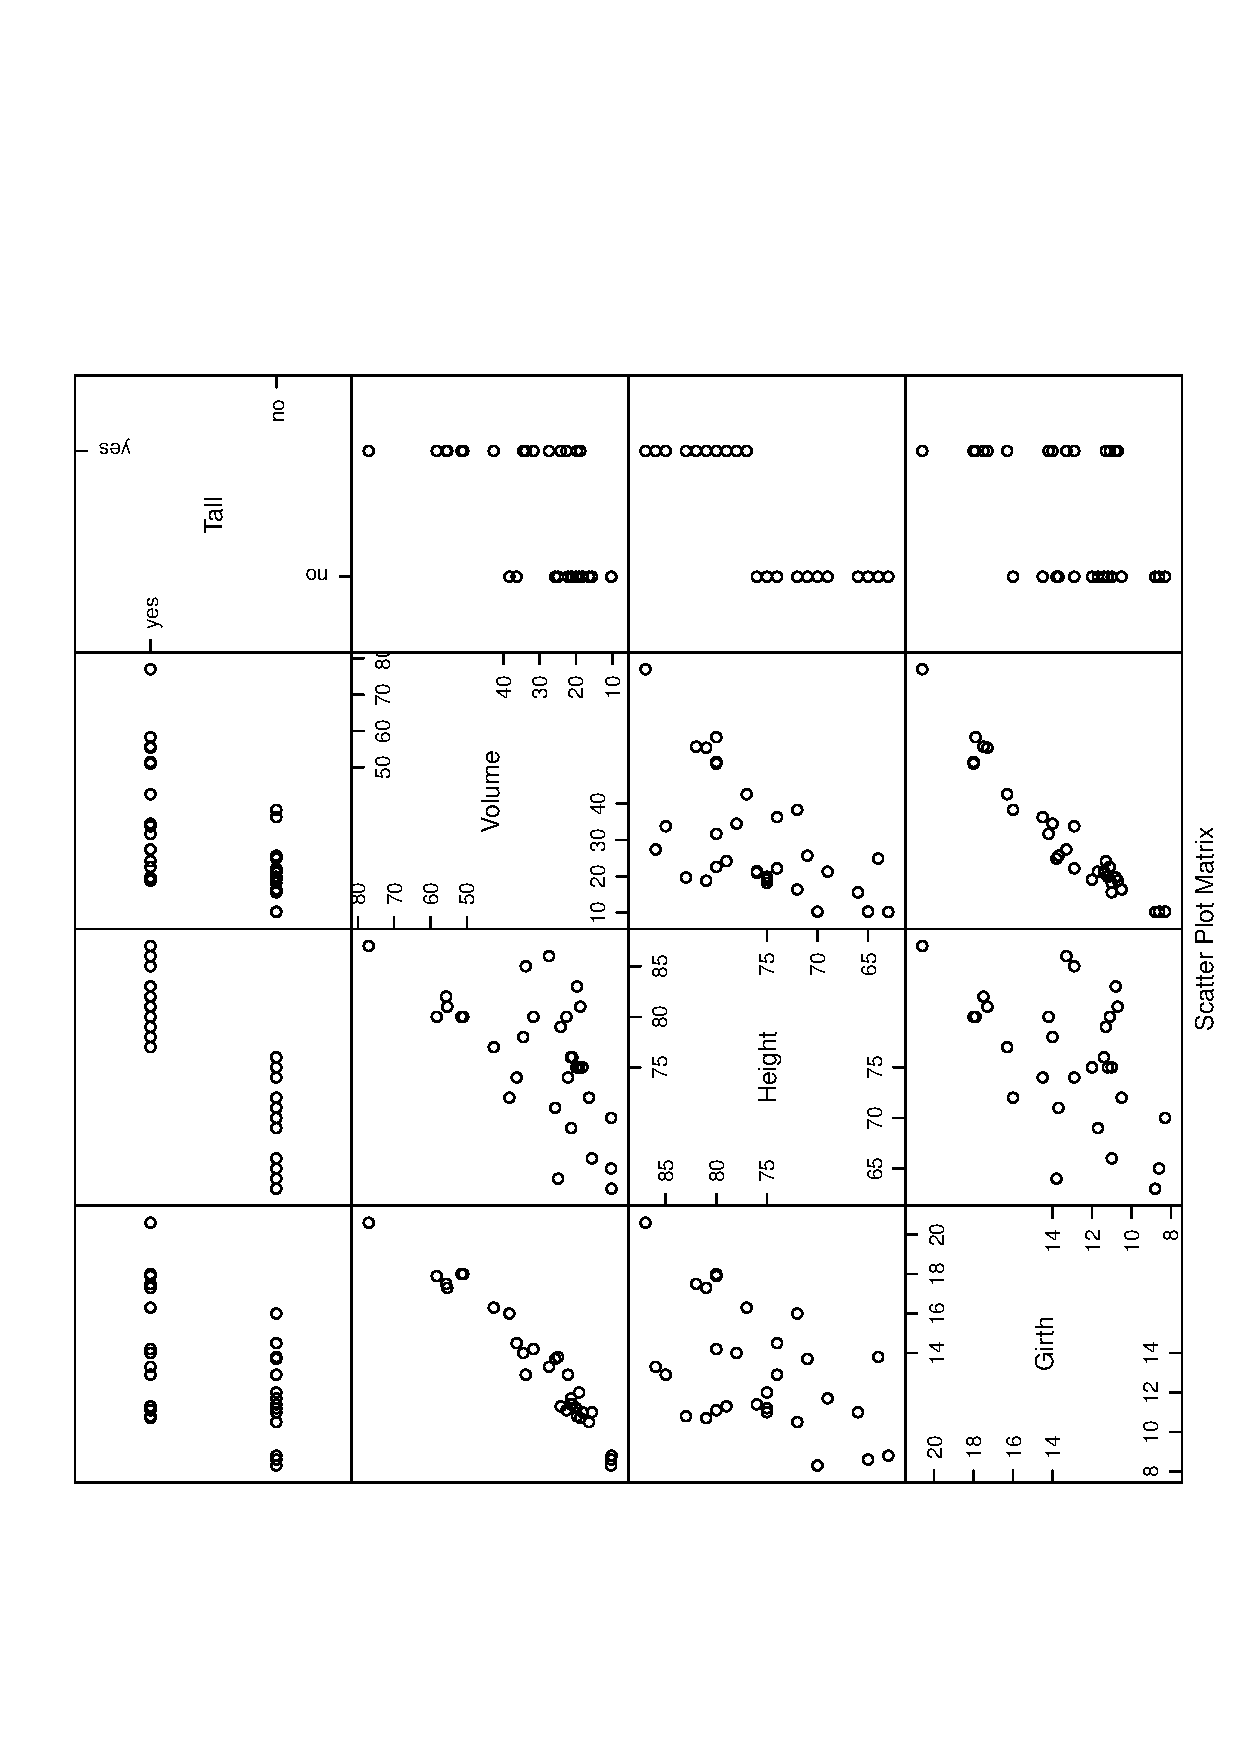
\includegraphics[width=5in, height=4in]{img/splom-trees.pdf}
    \caption[Scatterplot matrix of \texttt{trees} data]{\small A scatterplot matrix of \texttt{trees} data.}
    \label{fig:splom-trees}
  \end{figure}

The dependent (response) variable \texttt{Volume} is listed in the first row of the scatterplot matrix. Moving from left to right, we see an approximately linear relationship between \texttt{Volume} and the independent (explanatory) variables \texttt{Height} and \texttt{Girth}. A first guess at a model for these data might be
\begin{equation}
Y=\beta_{0}+\beta_{1}x_{1}+\beta_{2}x_{2}+\epsilon,
\end{equation}
in which case the quantity $\mu(x_{1},x_{2})=\beta_{0}+\beta_{1}x_{1}+\beta_{2}x_{2}$ would represent the mean value of $Y$ at the point $(x_{1},x_{2})$.
\end{example}
\subsection{What does it mean?}
\label{sec-1-1-1}


The interpretation is simple. The intercept $\beta_{0}$ represents the mean \texttt{Volume} when all other independent variables are zero. The parameter $\beta_{i}$ represents the change in mean \texttt{Volume} when there is a unit increase in $x_{i}$, while the other independent variable is held constant. For the \texttt{trees} data, $\beta_{1}$ represents the change in average \texttt{Volume} as \texttt{Girth} increases by one unit when the \texttt{Height} is held constant, and $\beta_{2}$ represents the change in average \texttt{Volume} as \texttt{Height} increases by one unit when the \texttt{Girth} is held constant. 


In simple linear regression, we had one independent variable and our linear regression surface was 1D, simply a line. In multiple regression there are many independent variables and so our linear regression surface will be many-D\ldots{} in general, a hyperplane. But when there are only two explanatory variables the hyperplane is just an ordinary plane and we can look at it with a 3D scatterplot. 

One way to do this is with the \textsf{R} Commander in the \texttt{Rcmdr} package \cite{Foxrcmdr}. It has a 3D scatterplot option under the \textsf{Graphs} menu. It is especially great because the resulting graph is dynamic; it can be moved around with the mouse, zoomed, \emph{etc}. But that particular display does not translate well to a printed book.

Another way to do it is with the \texttt{scatterplot3d} function in the \texttt{scatterplot3d} package. The code follows, and the result is shown in Figure \ref{fig:3D-scatterplot-trees}.


\begin{verbatim}
library(scatterplot3d)
s3d <- with(trees, scatterplot3d(Girth, Height, Volume, 
                                 pch = 16, highlight.3d = TRUE, 
                                 angle = 60))
fit <- lm(Volume ~ Girth + Height, data = trees)
\end{verbatim}



\begin{figure}[ht!]
    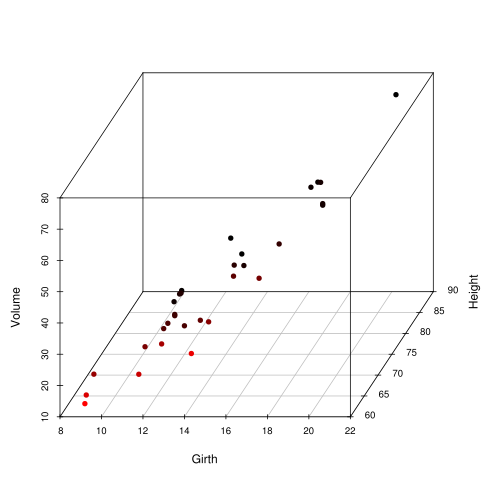
\includegraphics[width=5in, height=4in]{img/3D-scatterplot-trees.pdf}
    \caption[3D scatterplot with regression plane for the \texttt{trees} data]{\small A 3D scatterplot with regression plane for the \texttt{trees} data.}
    \label{fig:3D-scatterplot-trees}
  \end{figure}

Looking at the graph we see that the data points fall close to a plane in three dimensional space. (The plot looks remarkably good. In the author's experience it is rare to see points fit so well to the plane without some additional work.)
\section{Estimation and Prediction}
\label{sec-1-2}

\label{sec:Estimation-and-Prediction-MLR}
\subsection{Parameter estimates}
\label{sec-1-2-1}

\label{sub:mlr-parameter-estimates}

We will proceed exactly like we did in Section \ref{sec:SLR-Estimation}. We know
\begin{equation}
\upepsilon\sim\mathsf{mvnorm}\left(\mathtt{mean}=\mathbf{0}_{\mathrm{n}\times1},\,\mathtt{sigma}=\sigma^{2}\mathbf{I}_{\mathrm{n}\times\mathrm{n}}\right),
\end{equation}
which means that $\mathbf{Y}=\mathbf{X}\upbeta+\upepsilon$ has an $\mathsf{mvnorm}\left(\mathtt{mean}=\mathbf{X}\upbeta,\,\mathtt{sigma}=\sigma^{2}\mathbf{I}_{\mathrm{n}\times\mathrm{n}}\right)$ distribution. Therefore, the likelihood function\index{likelihood function} is
\begin{equation}
L(\upbeta,\sigma)=\frac{1}{2\pi^{n/2}\sigma}\exp\left\{ -\frac{1}{2\sigma^{2}}\left(\mathbf{Y}-\mathbf{X}\upbeta\right)^{\mathrm{T}}\left(\mathbf{Y}-\mathbf{X}\upbeta\right)\right\}.
\end{equation}

To \emph{maximize} the likelihood\index{maximum likelihood} in $\upbeta$, we need to \emph{minimize} the quantity $g(\upbeta)=\left(\mathbf{Y}-\mathbf{X}\upbeta\right)^{\mathrm{T}}\left(\mathbf{Y}-\mathbf{X}\upbeta\right)$. We do this by differentiating $g$ with respect to $\upbeta$. (It may be a good idea to brush up on the material in Appendices \ref{sec:Linear-Algebra} and \ref{sec:Multivariable-Calculus}.) First we will rewrite $g$:
\begin{equation}
g(\upbeta)=\mathbf{Y}^{\mathrm{T}}\mathbf{Y}-\mathbf{Y}^{\mathrm{T}}\mathbf{X}\upbeta-\upbeta^{\mathrm{T}}\mathbf{X}^{\mathrm{T}}\mathbf{Y}+\upbeta^{\mathrm{T}}\mathbf{X}^{\mathrm{T}}\mathbf{X}\upbeta,
\end{equation}
which can be further simplified to $g(\upbeta)=\mathbf{Y}^{\mathrm{T}}\mathbf{Y}-2\upbeta^{\mathrm{T}}\mathbf{X}^{\mathrm{T}}\mathbf{Y}+\upbeta^{\mathrm{T}}\mathbf{X}^{\mathrm{T}}\mathbf{X}\upbeta$ since $\upbeta^{\mathrm{T}}\mathbf{X}^{\mathrm{T}}\mathbf{Y}$ is $1\times1$ and thus equal to its transpose. Now we differentiate to get
\begin{equation}
\frac{\partial g}{\partial\upbeta}=\mathbf{0}-2\mathbf{X}^{\mathrm{T}}\mathbf{Y}+2\mathbf{X}^{\mathrm{T}}\mathbf{X}\upbeta,
\end{equation}
since $\mathbf{X}^{\mathrm{T}}\mathbf{X}$ is symmetric. Setting the derivative equal to the zero vector yields the so called ``normal equations''\index{normal equations}
\begin{equation}
\mathbf{X}^{\mathrm{T}}\mathbf{X}\upbeta=\mathbf{X}^{\mathrm{T}}\mathbf{Y}.
\end{equation}

In the case that $\mathbf{X}^{\mathrm{T}}\mathbf{X}$ is invertible
\footnote{We can find solutions of the normal equations even when $\mathbf{X}^{\mathrm{T}}\mathbf{X}$ is not of full rank, but the topic falls outside the scope of this book. The interested reader can consult an advanced text such as Rao \cite{Rao1999}.},
we may solve the equation for $\upbeta$ to get the maximum likelihood estimator of $\upbeta$ which we denote by $\mathbf{b}$:
\begin{equation}
\mathbf{b}=\left(\mathbf{X}^{\mathrm{T}}\mathbf{X}\right)^{-1}\mathbf{X}^{\mathrm{T}}\mathbf{Y}.\label{eq:b-formula-matrix}
\end{equation}

\begin{rem}
The formula in Equation \ref{eq:b-formula-matrix} is convenient for mathematical study but is inconvenient for numerical computation. Researchers have devised much more efficient algorithms for the actual calculation of the parameter estimates, and we do not explore them here.
\end{rem}

\begin{rem}
We have only found a critical value, and have not actually shown that the critical value is a minimum. We omit the details and refer the interested reader to \cite{Rao1999}.
\end{rem}

\paragraph*{How to do it with \textsf{R}}

We do all of the above just as we would in simple linear regression. The powerhouse is the \texttt{lm}\index{lm@\texttt{lm}} function. Everything else is based on it. We separate explanatory variables in the model formula by a plus sign.


\begin{verbatim}
trees.lm <- lm(Volume ~ Girth + Height, data = trees)
trees.lm
\end{verbatim}

\begin{verbatim}
 
 Call:
 lm(formula = Volume ~ Girth + Height, data = trees)
 
 Coefficients:
 (Intercept)        Girth       Height  
    -57.9877       4.7082       0.3393
\end{verbatim}

We see from the output that for the \texttt{trees} data our parameter estimates are 
\[
\mathbf{b}=\begin{bmatrix}-58.0 & 4.7 & 0.3\end{bmatrix},
\] 
and consequently our estimate of the mean response is $\hat{\mu}$ given by 
\begin{alignat}{1}
\hat{\mu}(x_{1},x_{2})= & \ b_{0}+b_{1}x_{1}+b_{2}x_{2},\\
\approx & -58.0+4.7x_{1}+0.3x_{2}.
\end{alignat}
We could see the entire model matrix $\mathbf{X}$ with the \texttt{model.matrix}\index{model.matrix@\texttt{model.matrix}} function, but in the interest of brevity we only show the first few rows. 


\begin{verbatim}
head(model.matrix(trees.lm))
\end{verbatim}

\begin{verbatim}
   (Intercept) Girth Height
 1           1   8.3     70
 2           1   8.6     65
 3           1   8.8     63
 4           1  10.5     72
 5           1  10.7     81
 6           1  10.8     83
\end{verbatim}
\subsection{Point Estimates of the Regression Surface}
\label{sec-1-2-2}

\label{sub:mlr-point-est-regsurface}

The parameter estimates $\mathbf{b}$ make it easy to find the fitted values\index{fitted values}, $\hat{\mathbf{Y}}$. We write them individually as $\hat{Y}_{i}$, $i=1,2,\ldots,n$, and recall that they are defined by
\begin{eqnarray}
\hat{Y}_{i} & = & \hat{\mu}(x_{1i},x_{2i}),\\
 & = & b_{0}+b_{1}x_{1i}+b_{2}x_{2i},\quad i=1,2,\ldots,n.
\end{eqnarray}
They are expressed more compactly by the matrix equation
\begin{equation}
\hat{\mathbf{Y}}=\mathbf{X}\mathbf{b}.
\end{equation}
From Equation \ref{eq:b-formula-matrix} we know that $\mathbf{b}=\left(\mathbf{X}^{\mathrm{T}}\mathbf{X}\right)^{-1}\mathbf{X}^{\mathrm{T}}\mathbf{Y}$, so we can rewrite
\begin{eqnarray}
\hat{\mathbf{Y}} & = & \mathbf{X}\left[\left(\mathbf{X}^{\mathrm{T}}\mathbf{X}\right)^{-1}\mathbf{X}^{\mathrm{T}}\mathbf{Y}\right],\\
 & = & \mathbf{H}\mathbf{Y},
\end{eqnarray}
where $\mathbf{H}=\mathbf{X}\left(\mathbf{X}^{\mathrm{T}}\mathbf{X}\right)^{-1}\mathbf{X}^{\mathrm{T}}$ is appropriately named \emph{the hat matrix}\index{hat matrix} because it ``puts the hat on $\mathbf{Y}$''. The hat matrix is very important in later courses. Some facts about $\mathbf{H}$ are
\begin{itemize}
\item $\mathbf{H}$ is a symmetric square matrix, of dimension $\mathrm{n}\times\mathrm{n}$.
\item The diagonal entries $h_{ii}$ satisfy $0\leq h_{ii}\leq1$ (compare to Equation \ref{eq:slr-leverage-between}).
\item The trace is $\mathrm{tr}(\mathbf{H})=p$.
\item $\mathbf{H}$ is \emph{idempotent} (also known as a \emph{projection matrix}) which means that $\mathbf{H}^{2}=\mathbf{H}$. The same is true of $\mathbf{I}-\mathbf{H}$.
\end{itemize}

Now let us write a column vector $\mathbf{x}_{0}=(x_{10},x_{20})^{\mathrm{T}}$ to denote given values of the explanatory variables \texttt{Girth =} $x_{10}$ and \texttt{Height =} $x_{20}$. These values may match those of the collected data, or they may be completely new values not observed in the original data set. We may use the parameter estimates to find $\hat{Y}(\mathbf{x}_{0})$, which will give us

\begin{enumerate}
\item an estimate of $\mu(\mathbf{x}_{0})$, the mean value of a future observation at $\mathbf{x}_{0}$, and
\item a prediction for $Y(\mathbf{x}_{0})$, the actual value of a future observation at $\mathbf{x}_{0}$.
\end{enumerate}

We can represent $\hat{Y}(\mathbf{x}_{0})$ by the matrix equation
\begin{equation}
\hat{Y}(\mathbf{x}_{0})=\mathbf{x}_{0}^{\mathrm{T}}\mathbf{b},\label{eq:mlr-single-yhat-matrix}
\end{equation}
which is just a fancy way to write
\begin{equation}
\hat{Y}(x_{10},x_{20})=b_{0}+b_{1}x_{10}+b_{2}x_{20}.
\end{equation}
 
\begin{example}
If we wanted to predict the average volume of black cherry trees that have \texttt{Girth = 15} in and are \texttt{Height = 77} ft tall then we would use the estimate 
\begin{alignat*}{1}
\hat{\mu}(15,\,77)= & -58+4.7(15)+0.3(77),\\
\approx & 35.6\mbox{\,\ ft}^{3}.
\end{alignat*}

We would use the same estimate $\hat{Y}=35.6$ to predict the measured \texttt{Volume} of another black cherry tree -- yet to be observed -- that has \texttt{Girth = 15} in and is \texttt{Height = 77} ft tall.
\end{example}

\paragraph*{How to do it with \textsf{R}}

The fitted values are stored inside \texttt{trees.lm} and may be accessed with the \texttt{fitted} function. We only show the first five fitted values.


\begin{verbatim}
fitted(trees.lm)[1:5]
\end{verbatim}

\begin{verbatim}
         1         2         3         4         5 
  4.837660  4.553852  4.816981 15.874115 19.869008
\end{verbatim}

The syntax for general prediction does not change much from simple linear regression. The computations are done with the \texttt{predict} function as described below. 

The only difference from SLR is in the way we tell \textsf{R} the values of the explanatory variables for which we want predictions. In SLR we had only one independent variable but in MLR we have many (for the \texttt{trees} data we have two). We will store values for the independent variables in the data frame \texttt{new}, which has two columns (one for each independent variable) and three rows (we shall make predictions at three different locations).


\begin{verbatim}
new <- data.frame(Girth = c(9.1, 11.6, 12.5), Height = c(69, 74, 87))
\end{verbatim}

We can view the locations at which we will predict:


\begin{verbatim}
new
\end{verbatim}

\begin{verbatim}
   Girth Height
 1   9.1     69
 2  11.6     74
 3  12.5     87
\end{verbatim}

We continue just like we would have done in SLR.


\begin{verbatim}
predict(trees.lm, newdata = new)
\end{verbatim}

\begin{verbatim}
         1         2         3 
  8.264937 21.731594 30.379205
\end{verbatim}



\begin{example}
Using the \texttt{trees} data,
\begin{enumerate}
\item Report a point estimate of the mean \texttt{Volume} of a tree of \texttt{Girth} 9.1 in and \texttt{Height} 69 ft.

   The fitted value for $x_{1}=9.1$ and $x_{2}=69$ is  8.3, so a point estimate would be  8.3 cubic feet.
\item Report a point prediction for and a 95\% prediction interval for the \texttt{Volume} of a hypothetical tree of \texttt{Girth} 12.5 in and \texttt{Height} 87 ft.

   The fitted value for $x_{1} = 12.5$ and $x_{2} = 87$ is  30.4, so a point prediction for the \texttt{Volume} is  30.4 cubic feet.
\end{enumerate}
\end{example}
\subsection{Mean Square Error and Standard Error}
\label{sec-1-2-3}

\label{sub:mlr-mse-se}

The residuals are given by
\begin{equation}
\mathbf{E}=\mathbf{Y}-\hat{\mathbf{Y}}=\mathbf{Y}-\mathbf{H}\mathbf{Y}=(\mathbf{I}-\mathbf{H})\mathbf{Y}.
\end{equation}
Now we can use Theorem \ref{thm:mvnorm-dist-matrix-prod} to see that the residuals are distributed
\begin{equation}
\mathbf{E}\sim\mathsf{mvnorm}(\mathtt{mean}=\mathbf{0},\,\mathtt{sigma}=\sigma^{2}(\mathbf{I}-\mathbf{H})),
\end{equation}
since $(\mathbf{I}-\mathbf{H})\mathbf{X}\upbeta=\mathbf{X}\upbeta-\mathbf{X}\upbeta=\mathbf{0}$ and $(\mathbf{I}-\mathbf{H})\,(\sigma^{2}\mathbf{I})\,(\mathbf{I}-\mathbf{H})^{\mathrm{T}}=\sigma^{2}(\mathbf{I}-\mathbf{H})^{2}=\sigma^{2}(\mathbf{I}-\mathbf{H})$. The sum of squared errors $SSE$ is just
\begin{equation}
SSE=\mathbf{E}^{\mathrm{T}}\mathbf{E}=\mathbf{Y}^{\mathrm{T}}(\mathbf{I}-\mathbf{H})(\mathbf{I}-\mathbf{H})\mathbf{Y}=\mathbf{Y}^{\mathrm{T}}(\mathbf{I}-\mathbf{H})\mathbf{Y}.
\end{equation}
Recall that in SLR we had two parameters ($\beta_{0}$ and $\beta_{1}$) in our regression model and we estimated $\sigma^{2}$ with $s^{2}=SSE/(n-2)$. In MLR, we have $p+1$ parameters in our regression model and we might guess that to estimate $\sigma^{2}$ we would use the \emph{mean square error} $S^{2}$ defined by 
\begin{equation}
S^{2}=\frac{SSE}{n-(p+1)}.
\end{equation}
That would be a good guess. The \emph{residual standard error} is $S=\sqrt{S^{2}}$.

\paragraph*{How to do it with \textsf{R}}

The residuals are also stored with \texttt{trees.lm} and may be accessed with the \texttt{residuals} function. We only show the first five residuals.


\begin{verbatim}
residuals(trees.lm)[1:5]
\end{verbatim}

\begin{verbatim}
          1          2          3          4          5 
  5.4623403  5.7461484  5.3830187  0.5258848 -1.0690084
\end{verbatim}

The \texttt{summary} function output (shown later) lists the \texttt{Residual Standard Error} which is just $S=\sqrt{S^{2}}$. It is stored in the \texttt{sigma} component of the \texttt{summary} object.


\begin{verbatim}
treesumry <- summary(trees.lm)
treesumry$sigma
\end{verbatim}

\begin{verbatim}
 [1] 3.881832
\end{verbatim}

For the \texttt{trees} data we find $s\approx$  3.882.
\subsection{Interval Estimates of the Parameters}
\label{sec-1-2-4}

\label{sub:mlr-interval-est-params}

We showed in Section \ref{sub:mlr-parameter-estimates} that $\mathbf{b}=\left(\mathbf{X}^{\mathrm{T}}\mathbf{X}\right)^{-1}\mathbf{X}^{\mathrm{T}}\mathbf{Y}$, which is really just a big matrix -- namely $\left(\mathbf{X}^{\mathrm{T}}\mathbf{X}\right)^{-1}\mathbf{X}^{\mathrm{T}}$ -- multiplied by $\mathbf{Y}$. It stands to reason that the sampling distribution of $\mathbf{b}$ would be intimately related to the distribution of $\mathbf{Y}$, which we assumed to be
\begin{equation}
\mathbf{Y}\sim\mathsf{mvnorm}\left(\mathtt{mean}=\mathbf{X}\upbeta,\,\mathtt{sigma}=\sigma^{2}\mathbf{I}\right).
\end{equation}
Now recall Theorem \ref{thm:mvnorm-dist-matrix-prod} that we said we were going to need eventually (the time is now). That proposition guarantees that
\begin{equation}
\mathbf{b}\sim\mathsf{mvnorm}\left(\mathtt{mean}=\upbeta,\,\mathtt{sigma}=\sigma^{2}\left(\mathbf{X}^{\mathrm{T}}\mathbf{X}\right)^{-1}\right),\label{eq:distn-b-mlr}
\end{equation}
since
\begin{equation}
\E\mathbf{b}=\left(\mathbf{X}^{\mathrm{T}}\mathbf{X}\right)^{-1}\mathbf{X}^{\mathrm{T}}(\mathbf{X}\upbeta)=\upbeta,
\end{equation}
and
\begin{equation}
\mbox{Var}(\mathbf{b})=\left(\mathbf{X}^{\mathrm{T}}\mathbf{X}\right)^{-1}\mathbf{X}^{\mathrm{T}}(\sigma^{2}\mathbf{I})\mathbf{X}\left(\mathbf{X}^{\mathrm{T}}\mathbf{X}\right)^{-1}=\sigma^{2}\left(\mathbf{X}^{\mathrm{T}}\mathbf{X}\right)^{-1},
\end{equation}
the first equality following because the matrix $\left(\mathbf{X}^{\mathrm{T}}\mathbf{X}\right)^{-1}$ is symmetric.

There is a lot that we can glean from Equation \ref{eq:distn-b-mlr}. First, it follows that the estimator $\mathbf{b}$ is unbiased (see Section \ref{sec:Point-Estimation-1}). Second, the variances of $b_{0}$, $b_{1}$, \ldots{}, $b_{n}$ are exactly the diagonal elements of $\sigma^{2}\left(\mathbf{X}^{\mathrm{T}}\mathbf{X}\right)^{-1}$, which is completely known except for that pesky parameter $\sigma^{2}$. Third, we can estimate the standard error of $b_{i}$ (denoted $S_{b_{i}}$) with the mean square error $S$ (defined in the previous section) multiplied by the corresponding diagonal element of $\left(\mathbf{X}^{\mathrm{T}}\mathbf{X}\right)^{-1}$. Finally, given estimates of the standard errors we may construct confidence intervals for $\beta_{i}$ with an interval that looks like
\begin{equation}
b_{i}\pm\mathsf{t}_{\alpha/2}(\mathtt{df}=n-p-1)S_{b_{i}}.
\end{equation}
The degrees of freedom for the Student's $t$ distribution
\footnote{We are taking great leaps over the mathematical details. In particular, we have yet to show that $s^{2}$ has a chi-square distribution and we have not even come close to showing that $b_{i}$ and $s_{b_{i}}$ are independent. But these are entirely outside the scope of the present book and the reader may rest assured that the proofs await in later classes. See C.R. Rao for more.}
are the same as the denominator of $S^{2}$. 

\paragraph*{How to do it with \textsf{R}}

To get confidence intervals for the parameters we need only use \texttt{confint}\index{confint@\texttt{confint}}:


\begin{verbatim}
confint(trees.lm)
\end{verbatim}

\begin{verbatim}
                    2.5 %      97.5 %
 (Intercept) -75.68226247 -40.2930554
 Girth         4.16683899   5.2494820
 Height        0.07264863   0.6058538
\end{verbatim}



For example, using the calculations above we say that for the regression model \texttt{Volume \textasciitilde{} Girth + Height} we are 95\% confident that the parameter $\beta_{1}$ lies somewhere in the interval [  4.2,  5.2 ].
\subsection{Confidence and Prediction Intervals}
\label{sec-1-2-5}


We saw in Section \ref{sub:mlr-point-est-regsurface} how to make point estimates of the mean value of additional observations and predict values of future observations, but how good are our estimates? We need confidence and prediction intervals to gauge their accuracy, and lucky for us the formulas look similar to the ones we saw in SLR.

In Equation \ref{eq:mlr-single-yhat-matrix} we wrote \( \hat{Y}(\mathbf{x}_{0})=\mathbf{x}_{0}^{\mathrm{T}}\mathbf{b} \), and in Equation \ref{eq:distn-b-mlr} we saw that
\begin{equation}
\mathbf{b}\sim\mathsf{mvnorm}\left(\mathtt{mean}=\upbeta,\,\mathtt{sigma}=\sigma^{2}\left(\mathbf{X}^{\mathrm{T}}\mathbf{X}\right)^{-1}\right).
\end{equation}
The following is therefore immediate from Theorem \ref{thm:mvnorm-dist-matrix-prod}:
\begin{equation}
\hat{Y}(\mathbf{x}_{0})\sim\mathsf{mvnorm}\left(\mathtt{mean}=\mathbf{x}_{0}^{\mathrm{T}}\upbeta,\,\mathtt{sigma}=\sigma^{2}\mathbf{x}_{0}^{\mathrm{T}}\left(\mathbf{X}^{\mathrm{T}}\mathbf{X}\right)^{-1}\mathbf{x}_{0}\right).
\end{equation}
It should be no surprise that confidence intervals for the mean value of a future observation at the location $\mathbf{x}_{0}=\begin{bmatrix}x_{10} & x_{20} & \ldots & x_{p0}\end{bmatrix}^{\mathrm{T}}$ are given by
\begin{equation}
\hat{Y}(\mathbf{x}_{0})\pm\mathsf{t}_{\alpha/2}(\mathtt{df}=n-p-1)\, S\sqrt{\mathbf{x}_{0}^{\mathrm{T}}\left(\mathbf{X}^{\mathrm{T}}\mathbf{X}\right)^{-1}\mathbf{x}_{0}}.
\end{equation}
Intuitively, $\mathbf{x}_{0}^{\mathrm{T}}\left(\mathbf{X}^{\mathrm{T}}\mathbf{X}\right)^{-1}\mathbf{x}_{0}$ measures the distance of $\mathbf{x}_{0}$ from the center of the data. The degrees of freedom in the Student's $t$ critical value are $n-(p+1)$ because we need to estimate $p+1$ parameters.

Prediction intervals for a new observation at $\mathbf{x}_{0}$ are given by
\begin{equation}
\hat{Y}(\mathbf{x}_{0})\pm\mathsf{t}_{\alpha/2}(\mathtt{df}=n-p-1)\, S\sqrt{1+\mathbf{x}_{0}^{\mathrm{T}}\left(\mathbf{X}^{\mathrm{T}}\mathbf{X}\right)^{-1}\mathbf{x}_{0}}.
\end{equation}
The prediction intervals are wider than the confidence intervals, just as in Section \ref{sub:slr-interval-est-regline}.


\paragraph*{How to do it with \textsf{R}}

The syntax is identical to that used in SLR, with the proviso that we need to specify values of the independent variables in the data frame \texttt{new} as we did in Section \ref{sub:slr-interval-est-regline} (which we repeat here for illustration).


\begin{verbatim}
new <- data.frame(Girth = c(9.1, 11.6, 12.5), Height = c(69, 74, 87))
\end{verbatim}

Confidence intervals are given by


\begin{verbatim}
predict(trees.lm, newdata = new, interval = "confidence")
\end{verbatim}

\begin{verbatim}
         fit      lwr      upr
 1  8.264937  5.77240 10.75747
 2 21.731594 20.11110 23.35208
 3 30.379205 26.90964 33.84877
\end{verbatim}



Prediction intervals are given by


\begin{verbatim}
predict(trees.lm, newdata = new, interval = "prediction")
\end{verbatim}

\begin{verbatim}
         fit         lwr      upr
 1  8.264937 -0.06814444 16.59802
 2 21.731594 13.61657775 29.84661
 3 30.379205 21.70364103 39.05477
\end{verbatim}



As before, the interval type is decided by the \texttt{interval} argument and the default confidence level is 95\% (which can be changed with the \texttt{level} argument).

\begin{example}
Using the \texttt{trees} data, 

\begin{enumerate}
\item Report a 95\% confidence interval for the mean \texttt{Volume} of a tree of \texttt{Girth} 9.1 in and \texttt{Height} 69 ft.

   The 95\% CI is given by \( [  5.8,  10.8 ] \), so with 95\% confidence the mean \texttt{Volume} lies somewhere between \(  5.8 \) cubic feet and \(  10.8 \) cubic feet.
\item Report a 95\% prediction interval for the \texttt{Volume} of a hypothetical tree of \texttt{Girth} 12.5 in and \texttt{Height} 87 ft.

   The 95\% prediction interval is given by [  26.9,  33.8 ], so with 95\% confidence we may assert that the hypothetical \texttt{Volume} of a tree of \texttt{Girth} 12.5 in and \texttt{Height} 87 ft would lie somewhere between  26.9 cubic feet and  33.8 feet.
\end{enumerate}

\end{example}
\section{Model Utility and Inference}
\label{sec-1-3}

\label{sec:Model-Utility-and-MLR}
\subsection{Multiple Coefficient of Determination}
\label{sec-1-3-1}


We saw in Section \ref{sub:mlr-mse-se} that the error sum of squares $SSE$ can be conveniently written in MLR as 
\begin{equation}
SSE=\mathbf{Y}^{\mathrm{T}}(\mathbf{I}-\mathbf{H})\mathbf{Y}.\label{eq:mlr-sse-matrix}
\end{equation}
It turns out that there are equally convenient formulas for the total sum of squares $SSTO$ and the regression sum of squares $SSR$. They are:
\begin{alignat}{1}
SSTO= & \mathbf{Y}^{\mathrm{T}}\left(\mathbf{I}-\frac{1}{n}\mathbf{J}\right)\mathbf{Y}\label{eq:mlr-ssto-matrix}
\end{alignat}
and
\begin{alignat}{1}
SSR= & \mathbf{Y}^{\mathrm{T}}\left(\mathbf{H}-\frac{1}{n}\mathbf{J}\right)\mathbf{Y}.\label{eq:mlr-ssr-matrix}
\end{alignat}
(The matrix $\mathbf{J}$ is defined in Appendix \ref{sec:Linear-Algebra}.) Immediately from Equations \ref{eq:mlr-sse-matrix}, \ref{eq:mlr-ssto-matrix}, and \ref{eq:mlr-ssr-matrix} we get the \emph{Anova Equality}
\begin{equation} 
SSTO=SSE+SSR.
\end{equation}
(See Exercise \ref{xca:anova-equality}.) We define the \emph{multiple coefficient of determination} by the formula
\begin{equation} 
R^{2}=1-\frac{SSE}{SSTO}.
\end{equation}

We interpret $R^{2}$ as the proportion of total variation that is explained by the multiple regression model. In MLR we must be careful, however, because the value of $R^{2}$ can be artificially inflated by the addition of explanatory variables to the model, regardless of whether or not the added variables are useful with respect to prediction of the response variable. In fact, it can be proved that the addition of a single explanatory variable to a regression model will increase the value of $R^{2}$, \emph{no matter how worthless} the explanatory variable is. We could model the height of the ocean tides, then add a variable for the length of cheetah tongues on the Serengeti plain, and our $R^{2}$ would inevitably increase. 

This is a problem, because as the philosopher, Occam, once said: ``causes should not be multiplied beyond necessity''. We address the problem by penalizing $R^{2}$ when parameters are added to the model. The result is an \emph{adjusted} $R^{2}$ which we denote by $\overline{R}^{2}$.
\begin{equation}
\overline{R}^{2}=\left(R^{2}-\frac{p}{n-1}\right)\left(\frac{n-1}{n-p-1}\right).
\end{equation}
It is good practice for the statistician to weigh both $R^{2}$ and $\overline{R}^{2}$ during assessment of model utility. In many cases their values will be very close to each other. If their values differ substantially, or if one changes dramatically when an explanatory variable is added, then (s)he should take a closer look at the explanatory variables in the model.

\paragraph*{How to do it with \textsf{R}}
For the \texttt{trees} data, we can get $R^{2}$ and $\overline{R}^{2}$ from the \texttt{summary} output or access the values directly by name as shown (recall that we stored the \texttt{summary} object in \texttt{treesumry}).


\begin{verbatim}
treesumry$r.squared
\end{verbatim}

\begin{verbatim}
 [1] 0.94795
\end{verbatim}


\begin{verbatim}
treesumry$adj.r.squared
\end{verbatim}

\begin{verbatim}
 [1] 0.9442322
\end{verbatim}

High values of \(R^{2}\) and \( \overline{R}^2 \) such as these indicate that the model fits very well, which agrees with what we saw in Figure \ref{fig:3D-scatterplot-trees}.
\subsection{Overall \emph{F}-Test}
\label{sec-1-3-2}

\label{sub:mlr-Overall-F-Test}

Another way to assess the model's utility is to to test the hypothesis
\[
H_{0}:\beta_{1}=\beta_{2}=\cdots=\beta_{p}=0\mbox{ versus }H_{1}:\mbox{ at least one \ensuremath{\beta_{i}\neq0}}.
\]
The idea is that if all $\beta_{i}$'s were zero, then the explanatory variables $X_{1},\ldots,X_{p}$ would be worthless predictors for the response variable $Y$. We can test the above hypothesis with the overall $F$ statistic, which in MLR is defined by
\begin{equation}
F=\frac{SSR/p}{SSE/(n-p-1)}.
\end{equation}
When the regression assumptions hold and under $H_{0}$, it can be shown that $F\sim\mathsf{f}(\mathtt{df1}=p,\,\mathtt{df2}=n-p-1)$. We reject $H_{0}$ when $F$ is large, that is, when the explained variation is large relative to the unexplained variation.

\paragraph*{How to do it with \textsf{R}}

The overall $F$ statistic and its associated \emph{p}-value is listed at the bottom of the \texttt{summary} output, or we can access it directly by name; it is stored in the \texttt{fstatistic} component of the \texttt{summary} object. 


\begin{verbatim}
treesumry$fstatistic
\end{verbatim}

\begin{verbatim}
    value    numdf    dendf 
 254.9723   2.0000  28.0000
\end{verbatim}

For the \texttt{trees} data, we see that \( F =  254.972337410669 \) with a \emph{p}-value \texttt{< 2.2e-16}. Consequently we reject $H_{0}$, that is, the data provide strong evidence that not all $\beta_{i}$'s are zero.
\subsection{Student's \emph{t} Tests}
\label{sec-1-3-3}

\label{sub:mlr-Student's-t-Tests}

We know that
\begin{equation}
\mathbf{b}\sim\mathsf{mvnorm}\left(\mathtt{mean}=\upbeta,\,\mathtt{sigma}=\sigma^{2}\left(\mathbf{X}^{\mathrm{T}}\mathbf{X}\right)^{-1}\right)
\end{equation}
and we have seen how to test the hypothesis $H_{0}:\beta_{1}=\beta_{2}=\cdots=\beta_{p}=0$, but let us now consider the test
\begin{equation}
H_{0}:\beta_{i}=0\mbox{ versus }H_{1}:\beta_{i}\neq0,
\end{equation}
where $\beta_{i}$ is the coefficient for the \(i^{\textrm{th}}\) independent variable. We test the hypothesis by calculating a statistic, examining it's null distribution, and rejecting $H_{0}$ if the \emph{p-value} is small. If $H_{0}$ is rejected, then we conclude that there is a significant relationship between $Y$ and $x_{i}$ \emph{in the regression model} $Y\sim(x_{1},\ldots,x_{p})$. This last part of the sentence is very important because the significance of the variable $x_{i}$ sometimes depends on the presence of other independent variables in the model
\footnote{In other words, a variable might be highly significant one moment but then fail to be significant when another variable is added to the model. When this happens it often indicates a problem with the explanatory variables, such as /multicollinearity/. See Section \ref{sub:Multicollinearity}.}.

To test the hypothesis we go to find the sampling distribution of \( b_{i} \), the estimator of the corresponding parameter \( \beta_{i} \), when the null hypothesis is true. We saw in Section \ref{sub:mlr-interval-est-params} that 
\begin{equation}
T_{i}=\frac{b_{i}-\beta_{i}}{S_{b_{i}}}
\end{equation}
has a Student's $t$ distribution with $n-(p+1)$ degrees of freedom. (Remember, we are estimating $p+1$ parameters.) Consequently, under the null hypothesis $H_{0}:\beta_{i}=0$ the statistic $t_{i}=b_{i}/S_{b_{i}}$ has a $\mathsf{t}(\mathtt{df}=n-p-1)$ distribution.


\paragraph*{How to do it with \textsf{R}}

The Student's $t$ tests for significance of the individual explanatory variables are shown in the \texttt{summary} output.


\begin{verbatim}
treesumry
\end{verbatim}


\begin{verbatim}

Call:
lm(formula = Volume ~ Girth + Height, data = trees)

Residuals:
    Min      1Q  Median      3Q     Max 
-6.4065 -2.6493 -0.2876  2.2003  8.4847 

Coefficients:
            Estimate Std. Error t value Pr(>|t|)    
(Intercept) -57.9877     8.6382  -6.713 2.75e-07 ***
Girth         4.7082     0.2643  17.816  < 2e-16 ***
Height        0.3393     0.1302   2.607   0.0145 *  
---
Signif. codes:  0 '***' 0.001 '**' 0.01 '*' 0.05 '.' 0.1 ' ' 1 

Residual standard error: 3.882 on 28 degrees of freedom
Multiple R-squared: 0.948,	Adjusted R-squared: 0.9442 
F-statistic:   255 on 2 and 28 DF,  p-value: < 2.2e-16
\end{verbatim}

We see from the \emph{p-values} that there is a significant linear relationship between \texttt{Volume} and \texttt{Girth} and between \texttt{Volume} and \texttt{Height} in the regression model \texttt{Volume \textasciitilde{} Girth + Height}. Further, it appears that the \texttt{Intercept} is significant in the aforementioned model.
\section{Polynomial Regression}
\label{sec-1-4}

\label{sec:Polynomial-Regression}
\subsection{Quadratic Regression Model}
\label{sec-1-4-1}


In each of the previous sections we assumed that $\mu$ was a linear function of the explanatory variables. For example, in SLR we assumed that $\mu(x)=\beta_{0}+\beta_{1}x$, and in our previous MLR examples we assumed $\mu(x_{1},x_{2})=\beta_{0}+\beta_{1}x_{1}+\beta_{2}x_{2}$. In every case the scatterplots indicated that our assumption was reasonable. Sometimes, however, plots of the data suggest that the linear model is incomplete and should be modified.


\begin{verbatim}
qplot(Girth, Volume, data = trees)
\end{verbatim}



\begin{figure}[ht!]
    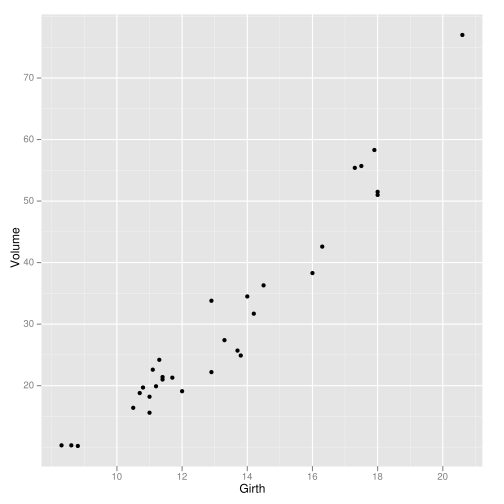
\includegraphics[width=5in, height=4in]{img/Scatterplot-Volume-Girth-trees.pdf}
    \caption[Scatterplot of \texttt{Volume} versus \texttt{Girth} for the \texttt{trees} data]{\small A scatterplot of \texttt{Volume} versus \texttt{Girth} for the \texttt{trees} data.}
    \label{fig:Scatterplot-Volume-Girth-trees}
  \end{figure}

For example, let us examine a scatterplot of \texttt{Volume} versus \texttt{Girth} a little more closely. See Figure \ref{fig:Scatterplot-Volume-Girth-trees}. There might be a slight curvature to the data; the volume curves ever so slightly upward as the girth increases. After looking at the plot we might try to capture the curvature with a mean response such as 
\begin{equation}
\mu(x_{1})=\beta_{0}+\beta_{1}x_{1}+\beta_{2}x_{1}^{2}.
\end{equation}
The model associated with this choice of $\mu$ is
\begin{equation}
Y=\beta_{0}+\beta_{1}x_{1}+\beta_{2}x_{1}^{2}+\epsilon.
\end{equation}
The regression assumptions are the same. Almost everything indeed is the same. In fact, it is still called a ``linear regression model'', since the mean response $\mu$ is linear \emph{in the parameters} $\beta_{0}$, $\beta_{1}$, and $\beta_{2}$. 

\textbf{However, there is one important difference.} When we introduce the squared variable in the model we inadvertently also introduce strong dependence between the terms which can cause significant numerical problems when it comes time to calculate the parameter estimates. Therefore, we should usually rescale the independent variable to have mean zero (and even variance one if we wish) \textbf{before} fitting the model. That is, we replace the $x_{i}$'s with $x_{i}-\overline{x}$ (or $(x_{i}-\overline{x})/s$) before fitting the model
\footnote{Rescaling the data gets the job done but a better way to avoid the multicollinearity introduced by the higher order terms is with /orthogonal polynomials/, whose coefficients are chosen just right so that the polynomials are not correlated with each other. This is beginning to linger outside the scope of this book, however, so we will content ourselves with a brief mention and then stick with the rescaling approach in the discussion that follows. A nice example of orthogonal polynomials in action can be run with \texttt{example(cars)}.}.

\paragraph*{How to do it with \textsf{R}}

There are multiple ways to fit a quadratic model to the variables \texttt{Volume} and \texttt{Girth} using \textsf{R}.
\begin{enumerate}
\item One way would be to square the values for \texttt{Girth} and save them in a vector \texttt{Girthsq}. Next, fit the linear model \texttt{Volume \textasciitilde{} Girth + Girthsq}.
\item A second way would be to use the \emph{insulate} function in \textsf{R}, denoted by \texttt{I}:
\begin{verbatim}
    Volume ~ Girth + I(Girth^2)
\end{verbatim}
\end{enumerate}
The second method is shorter than the first but the end result is the same. And once we calculate and store the fitted model (in, say, \texttt{treesquad.lm}) all of the previous comments regarding \textsf{R} apply.  
\begin{enumerate}
\item A third and ``right'' way to do it is with orthogonal polynomials:
\begin{verbatim}
     Volume ~ poly(Girth, degree = 2)
\end{verbatim}
   See \texttt{?poly} and \texttt{?cars} for more information. Note that we can recover the approach in 2 with \texttt{poly(Girth, degree = 2, raw = TRUE)}.
\end{enumerate}

\begin{example}
We will fit the quadratic model to the \texttt{trees} data and display the results with \texttt{summary}, being careful to rescale the data before fitting the model. We may rescale the \texttt{Girth} variable to have zero mean and unit variance on-the-fly with the \texttt{scale} function.


\begin{verbatim}
treesquad.lm <- lm(Volume ~ scale(Girth) + I(scale(Girth)^2),                    data = trees)
summary(treesquad.lm)
\end{verbatim}


\begin{verbatim}

Call:
lm(formula = Volume ~ scale(Girth) + I(scale(Girth)^2), data = trees)

Residuals:
    Min      1Q  Median      3Q     Max 
-5.4889 -2.4293 -0.3718  2.0764  7.6447 

Coefficients:
                  Estimate Std. Error t value Pr(>|t|)    
(Intercept)        27.7452     0.8161  33.996  < 2e-16 ***
scale(Girth)       14.5995     0.6773  21.557  < 2e-16 ***
I(scale(Girth)^2)   2.5067     0.5729   4.376 0.000152 ***
---
Signif. codes:  0 '***' 0.001 '**' 0.01 '*' 0.05 '.' 0.1 ' ' 1 

Residual standard error: 3.335 on 28 degrees of freedom
Multiple R-squared: 0.9616,	Adjusted R-squared: 0.9588 
F-statistic: 350.5 on 2 and 28 DF,  p-value: < 2.2e-16
\end{verbatim}

We see that the $F$ statistic indicates the overall model including \texttt{Girth} and \texttt{Girth\textasciicircum{}2} is significant. Further, there is strong evidence that both \texttt{Girth} and \texttt{Girth\textasciicircum{}2} are significantly related to \texttt{Volume}. We may examine a scatterplot together with the fitted quadratic function using the \texttt{lines} function, which adds a line to the plot tracing the estimated mean response.



\begin{verbatim}
a <- ggplot(trees, aes(scale(Girth), Volume))
a + stat_smooth(method = lm, formula = y ~ poly(x, 2)) + geom_point()
\end{verbatim}



\begin{figure}[ht!]
    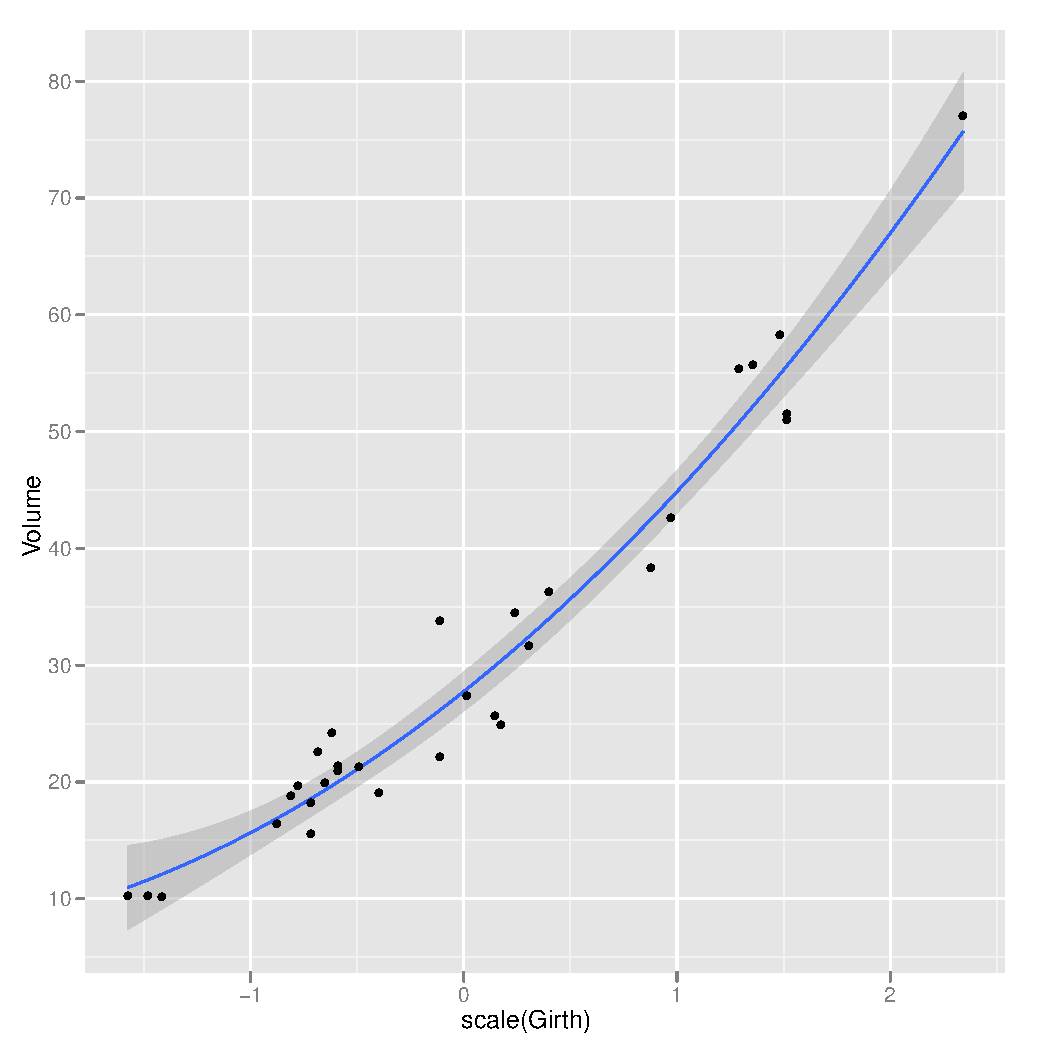
\includegraphics[width=5in, height=4in]{img/Fitting-the-Quadratic.pdf}
    \caption[Quadratic model for the \texttt{trees} data]{\small A quadratic model for the \texttt{trees} data.}
    \label{fig:Fitting-the-Quadratic}
  \end{figure}

The plot is shown in Figure \ref{fig:Fitting-the-Quadratic}. Pay attention to the scale on the $x$-axis: it is on the scale of the transformed \texttt{Girth} data and not on the original scale.

\end{example}


\begin{rem}
When a model includes a quadratic term for an independent variable, it is customary to also include the linear term in the model. The principle is called \emph{parsimony}. More generally, if the researcher decides to include $x^{m}$ as a term in the model, then (s)he should also include all lower order terms $x$, $x^{2}$, \ldots{},$x^{m-1}$ in the model.
\end{rem}

We do estimation/prediction the same way that we did in Section \ref{sub:mlr-point-est-regsurface}, except we do not need a \texttt{Height} column in the dataframe \texttt{new} since the variable is not included in the quadratic model.


\begin{verbatim}
new <- data.frame(Girth = c(9.1, 11.6, 12.5))
predict(treesquad.lm, newdata = new, interval = "prediction")
\end{verbatim}

\begin{verbatim}
        fit       lwr      upr
 1 11.56982  4.347426 18.79221
 2 20.30615 13.299050 27.31325
 3 25.92290 18.972934 32.87286
\end{verbatim}

The predictions and intervals are slightly different from what they were previously. Notice that it was not necessary to rescale the \texttt{Girth} prediction data before input to the \texttt{predict} function; the model did the rescaling for us automatically.

\begin{rem}
We have mentioned on several occasions that it is important to rescale the explanatory variables for polynomial regression. Watch what happens if we ignore this advice:


\begin{verbatim}
summary(lm(Volume ~ Girth + I(Girth^2), data = trees))
\end{verbatim}


\begin{verbatim}

Call:
lm(formula = Volume ~ Girth + I(Girth^2), data = trees)

Residuals:
    Min      1Q  Median      3Q     Max 
-5.4889 -2.4293 -0.3718  2.0764  7.6447 

Coefficients:
            Estimate Std. Error t value Pr(>|t|)    
(Intercept) 10.78627   11.22282   0.961 0.344728    
Girth       -2.09214    1.64734  -1.270 0.214534    
I(Girth^2)   0.25454    0.05817   4.376 0.000152 ***
---
Signif. codes:  0 '***' 0.001 '**' 0.01 '*' 0.05 '.' 0.1 ' ' 1 

Residual standard error: 3.335 on 28 degrees of freedom
Multiple R-squared: 0.9616,	Adjusted R-squared: 0.9588 
F-statistic: 350.5 on 2 and 28 DF,  p-value: < 2.2e-16
\end{verbatim}

Now nothing is significant in the model except \texttt{Girth\textasciicircum{}2}. We could delete the \texttt{Intercept} and \texttt{Girth} from the model, but the model would no longer be \emph{parsimonious}. A novice may see the output and be confused about how to proceed, while the seasoned statistician recognizes immediately that \texttt{Girth} and \texttt{Girth\textasciicircum{}2} are highly correlated (see Section \ref{sub:Multicollinearity}). The only remedy to this ailment is to rescale \texttt{Girth}, which we should have done in the first place.

In Example \ref{exa:mlr-trees-poly-no-rescale} of Section \ref{sec:Partial-F-Statistic} we investigate this issue further.

\end{rem}
\section{Interaction}
\label{sec-1-5}

\label{sec:Interaction}

In our model for tree volume there have been two independent variables: \texttt{Girth} and \texttt{Height}. We may suspect that the independent variables are related, that is, values of one variable may tend to influence values of the other. It may be desirable to include an additional term in our model to try and capture the dependence between the variables. Interaction terms are formed by multiplying one (or more) explanatory variable(s) by another. 


\begin{example}
Perhaps the \texttt{Girth} and \texttt{Height} of the tree interact to influence the its \texttt{Volume}; we would like to investigate whether the model (\texttt{Girth} = $x_{1}$ and \texttt{Height} = $x_{2}$) 
\begin{equation}
Y=\beta_{0}+\beta_{1}x_{1}+\beta_{2}x_{2}+\epsilon
\end{equation}
would be significantly improved by the model
\begin{equation}
Y=\beta_{0}+\beta_{1}x_{1}+\beta_{2}x_{2}+\beta_{1:2}x_{1}x_{2}+\epsilon,
\end{equation}
where the subscript $1:2$ denotes that $\beta_{1:2}$ is a coefficient
of an interaction term between $x{}_{1}$ and $x_{2}$. 

\end{example}

\paragraph*{What does it mean?}

Consider the mean response $\mu(x_{1},x_{2})$ as a function of $x_{2}$:
\begin{equation}
\mu(x_{2})=(\beta_{0}+\beta_{1}x_{1})+\beta_{2}x_{2}.
\end{equation}
This is a linear function of $x_{2}$ with slope $\beta_{2}$. As $x_{1}$ changes, the $y$-intercept of the mean response in $x_{2}$ changes, but the slope remains the same. Therefore, the mean response in $x_{2}$ is represented by a collection of parallel lines all with common slope $\beta_{2}$.

Now think about what happens when the interaction term $\beta_{1:2}x_{1}x_{2}$ is included. The mean response in $x_{2}$ now looks like
\begin{equation}
\mu(x_{2})=(\beta_{0}+\beta_{1}x_{1})+(\beta_{2}+\beta_{1:2}x_{1})x_{2}.
\end{equation}
In this case we see that not only the $y$-intercept changes when $x_{1}$ varies, but the slope also changes in $x_{1}$. Thus, the interaction term allows the slope of the mean response in $x_{2}$ to increase and decrease as $x_{1}$ varies. 

\paragraph*{How to do it with \textsf{R}}

There are several ways to introduce an interaction term into the model.
\begin{enumerate}
\item Make a new variable \texttt{prod <- Girth * Height}, then include \texttt{prod} in the model formula \texttt{Volume \textasciitilde{} Girth + Height + prod}. This method is perhaps the most transparent, but it also reserves memory space unnecessarily.
\item Once can construct an interaction term directly in \textsf{R} with a colon ``=:=''. For this example, the model formula would look like 
\begin{verbatim}
    Volume ~ Girth + Height + Girth:Height
\end{verbatim}
\end{enumerate}

For the \texttt{trees} data, we fit the model with the interaction using method two and see if it is significant:


\begin{verbatim}
treesint.lm <- lm(Volume ~ Girth + Height + Girth:Height, data = trees)
summary(treesint.lm)
\end{verbatim}


\begin{verbatim}

Call:
lm(formula = Volume ~ Girth + Height + Girth:Height, data = trees)

Residuals:
    Min      1Q  Median      3Q     Max 
-6.5821 -1.0673  0.3026  1.5641  4.6649 

Coefficients:
             Estimate Std. Error t value Pr(>|t|)    
(Intercept)  69.39632   23.83575   2.911  0.00713 ** 
Girth        -5.85585    1.92134  -3.048  0.00511 ** 
Height       -1.29708    0.30984  -4.186  0.00027 ***
Girth:Height  0.13465    0.02438   5.524 7.48e-06 ***
---
Signif. codes:  0 '***' 0.001 '**' 0.01 '*' 0.05 '.' 0.1 ' ' 1 

Residual standard error: 2.709 on 27 degrees of freedom
Multiple R-squared: 0.9756,	Adjusted R-squared: 0.9728 
F-statistic: 359.3 on 3 and 27 DF,  p-value: < 2.2e-16
\end{verbatim}

We can see from the output that the interaction term is highly significant. Further, the estimate $b_{1:2}$ is positive. This means that the slope of $\mu(x_{2})$ is steeper for bigger values of \texttt{Girth}. Keep in mind: the same interpretation holds for $\mu(x_{1})$; that is, the slope of $\mu(x_{1})$ is steeper for bigger values of \texttt{Height}.

For the sake of completeness we calculate confidence intervals for the parameters and do prediction as before.


\begin{verbatim}
confint(treesint.lm)
\end{verbatim}

\begin{verbatim}
                    2.5 %      97.5 %
 (Intercept)  20.48938699 118.3032441
 Girth        -9.79810354  -1.9135923
 Height       -1.93282845  -0.6613383
 Girth:Height  0.08463628   0.1846725
\end{verbatim}


\begin{verbatim}
new <- data.frame(Girth = c(9.1, 11.6, 12.5), Height = c(69, 74, 87))
predict(treesint.lm, newdata = new, interval = "prediction")
\end{verbatim}

\begin{verbatim}
        fit       lwr      upr
 1 11.15884  5.236341 17.08134
 2 21.07164 15.394628 26.74866
 3 29.78862 23.721155 35.85608
\end{verbatim}

\begin{rem}
There are two other ways to include interaction terms in model formulas. For example, we could have written \texttt{Girth * Height} or even \texttt{(Girth + Height)\textasciicircum{}2} and both would be the same as \texttt{Girth + Height + Girth:Height}. 
\end{rem}

These examples can be generalized to more than two independent variables, say three, four, or even more. We may be interested in seeing whether any pairwise interactions are significant. We do this with a model formula that looks something like \texttt{y \textasciitilde{} (x1 + x2 + x3 + x4)\textasciicircum{}2}.  
\section{Qualitative Explanatory Variables}
\label{sec-1-6}

\label{sec:Qualitative-Explanatory-Variables}

We have so far been concerned with numerical independent variables taking values in a subset of real numbers. In this section, we extend our treatment to include the case in which one of the explanatory variables is qualitative, that is, a \emph{factor}. Qualitative variables take values in a set of \emph{levels}, which may or may not be ordered. See Section \ref{sub:Qualitative-Data}.

\begin{note*}
The \texttt{trees} data do not have any qualitative explanatory variables, so we will construct one for illustrative purposes
\footnote{This procedure of replacing a continuous variable by a discrete/qualitative one is called \emph{binning}, and is almost \emph{never} the right thing to do. We are in a bind at this point, however, because we have invested this chapter in the \texttt{trees} data and I do not want to switch mid-discussion. I am currently searching for a data set with pre-existing qualitative variables that also conveys the same points present in the trees data, and when I find it I will update this chapter accordingly.}.
We will leave the \texttt{Girth} variable alone, but we will replace the variable \texttt{Height} by a new variable \texttt{Tall} which indicates whether or not the cherry tree is taller than a certain threshold (which for the sake of argument will be the sample median height of 76 ft). That is, \texttt{Tall} will be defined by
\begin{equation}
\mathtt{Tall}=
\begin{cases}
\mathtt{yes}, & \mbox{if }\mathtt{Height}>76,\\
\mathtt{no}, & \mbox{if }\mathtt{Height}\leq76.
\end{cases}
\end{equation}

We can construct \texttt{Tall} very quickly in \textsf{R} with the \texttt{cut} function:


\begin{verbatim}
trees$Tall <- cut(trees$Height, breaks = c(-Inf, 76, Inf), 
                  labels = c("no","yes"))
trees$Tall[1:5]
\end{verbatim}

\begin{verbatim}
 [1] no  no  no  no  yes
 Levels: no yes
\end{verbatim}

Note that \texttt{Tall} is automatically generated to be a factor with the labels in the correct order. See \texttt{?cut} for more. 
\end{note*}

Once we have \texttt{Tall}, we include it in the regression model just like we would any other variable. It is handled internally in a special way. Define a ``dummy variable'' \texttt{Tallyes} that takes values
\begin{equation}
\mathtt{Tallyes}=
\begin{cases}
1, & \mbox{if }\mathtt{Tall}=\mathtt{yes},\\
0, & \mbox{otherwise.}
\end{cases}
\end{equation}
That is, \texttt{Tallyes} is an \emph{indicator variable} which indicates when a respective tree is tall. The model may now be written as 
\begin{equation}
\mathtt{Volume}=\beta_{0}+\beta_{1}\mathtt{Girth}+\beta_{2}\mathtt{Tallyes}+\epsilon.
\end{equation}
Let us take a look at what this definition does to the mean response. Trees with \texttt{Tall = yes} will have the mean response
\begin{equation}
\mu(\mathtt{Girth})=(\beta_{0}+\beta_{2})+\beta_{1}\mathtt{Girth},
\end{equation}
while trees with \texttt{Tall = no} will have the mean response
\begin{equation} 
\mu(\mathtt{Girth})=\beta_{0}+\beta_{1}\mathtt{Girth}.
\end{equation}
In essence, we are fitting two regression lines: one for tall trees, and one for short trees. The regression lines have the same slope but they have different $y$ intercepts (which are exactly $|\beta_{2}|$ far apart).

\paragraph*{How to do it with \textsf{R}}

The important thing is to double check that the qualitative variable in question is stored as a factor. The way to check is with the \texttt{class} command. For example,


\begin{verbatim}
class(trees$Tall)
\end{verbatim}

\begin{verbatim}
 [1] "factor"
\end{verbatim}

If the qualitative variable is not yet stored as a factor then we may convert it to one with the \texttt{factor} command. See Section \ref{sub:Qualitative-Data}. Other than this we perform MLR as we normally would.


\begin{verbatim}
treesdummy.lm <- lm(Volume ~ Girth + Tall, data = trees)
summary(treesdummy.lm)
\end{verbatim}


\begin{verbatim}

Call:
lm(formula = Volume ~ Girth + Tall, data = trees)

Residuals:
    Min      1Q  Median      3Q     Max 
-5.7788 -3.1710  0.4888  2.6737 10.0619 

Coefficients:
            Estimate Std. Error t value Pr(>|t|)    
(Intercept) -34.1652     3.2438  -10.53 3.02e-11 ***
Girth         4.6988     0.2652   17.72  < 2e-16 ***
Tall[T.yes]   4.3072     1.6380    2.63   0.0137 *  
---
Signif. codes:  0 '***' 0.001 '**' 0.01 '*' 0.05 '.' 0.1 ' ' 1 

Residual standard error: 3.875 on 28 degrees of freedom
Multiple R-squared: 0.9481,	Adjusted R-squared: 0.9444 
F-statistic: 255.9 on 2 and 28 DF,  p-value: < 2.2e-16
\end{verbatim}

From the output we see that all parameter estimates are statistically significant and we conclude that the mean response differs for trees with \texttt{Tall = yes} and trees with \texttt{Tall = no}.

\begin{rem}
We were somewhat disingenuous when we defined the dummy variable \texttt{Tallyes} because, in truth, \textsf{R} defines \texttt{Tallyes} automatically without input from the user
\footnote{That is, \textsf{R} by default handles contrasts according to its internal settings which may be customized by the user for fine control. Given that we will not investigate contrasts further in this book it does not serve the discussion to delve into those settings, either. The interested reader should check \texttt{?contrasts} for details.}. 
Indeed, the author fit the model beforehand and wrote the discussion afterward with the knowledge of what \textsf{R} would do so that the output the reader saw would match what (s)he had previously read. The way that \textsf{R} handles factors internally is part of a much larger topic concerning \emph{contrasts}, which falls outside the scope of this book. The interested reader should see Neter et al \cite{Neter1996} or Fox \cite{Fox1997} for more. 
\end{rem}

\begin{rem}
In general, if an explanatory variable \texttt{foo} is qualitative with $n$ levels \texttt{bar1}, \texttt{bar2}, \ldots{}, \texttt{barn} then \textsf{R} will by default automatically define $n-1$ indicator variables in the following way:
\begin{eqnarray*}
\mathtt{foobar2} & = & \begin{cases}
1, & \mbox{if }\mathtt{foo}=\mathtt{"bar2"},\\
0, & \mbox{otherwise.}\end{cases},\,\ldots,\,\mathtt{foobarn}=\begin{cases}
1, & \mbox{if }\mathtt{foo}=\mathtt{"barn"},\\
0, & \mbox{otherwise.}\end{cases}
\end{eqnarray*}
The level \texttt{bar1} is represented by $\mathtt{foobar2}=\cdots=\mathtt{foobarn}=0$. We just need to make sure that \texttt{foo} is stored as a factor and \textsf{R} will take care of the rest. 
\end{rem}
\subsection{Graphing the Regression Lines}
\label{sec-1-6-1}


We can see a plot of the two regression lines with the following mouthful of code.


\begin{verbatim}
treesTall <- split(trees, trees$Tall)
treesTall[["yes"]]$Fit <- predict(treesdummy.lm, treesTall[["yes"]])
treesTall[["no"]]$Fit <- predict(treesdummy.lm, treesTall[["no"]])
plot(Volume ~ Girth, data = trees, type = "n")
points(Volume ~ Girth, data = treesTall[["yes"]], pch = 1)
points(Volume ~ Girth, data = treesTall[["no"]], pch = 2)
lines(Fit ~ Girth, data = treesTall[["yes"]])
lines(Fit ~ Girth, data = treesTall[["no"]])
\end{verbatim}



\begin{figure}[ht!]
    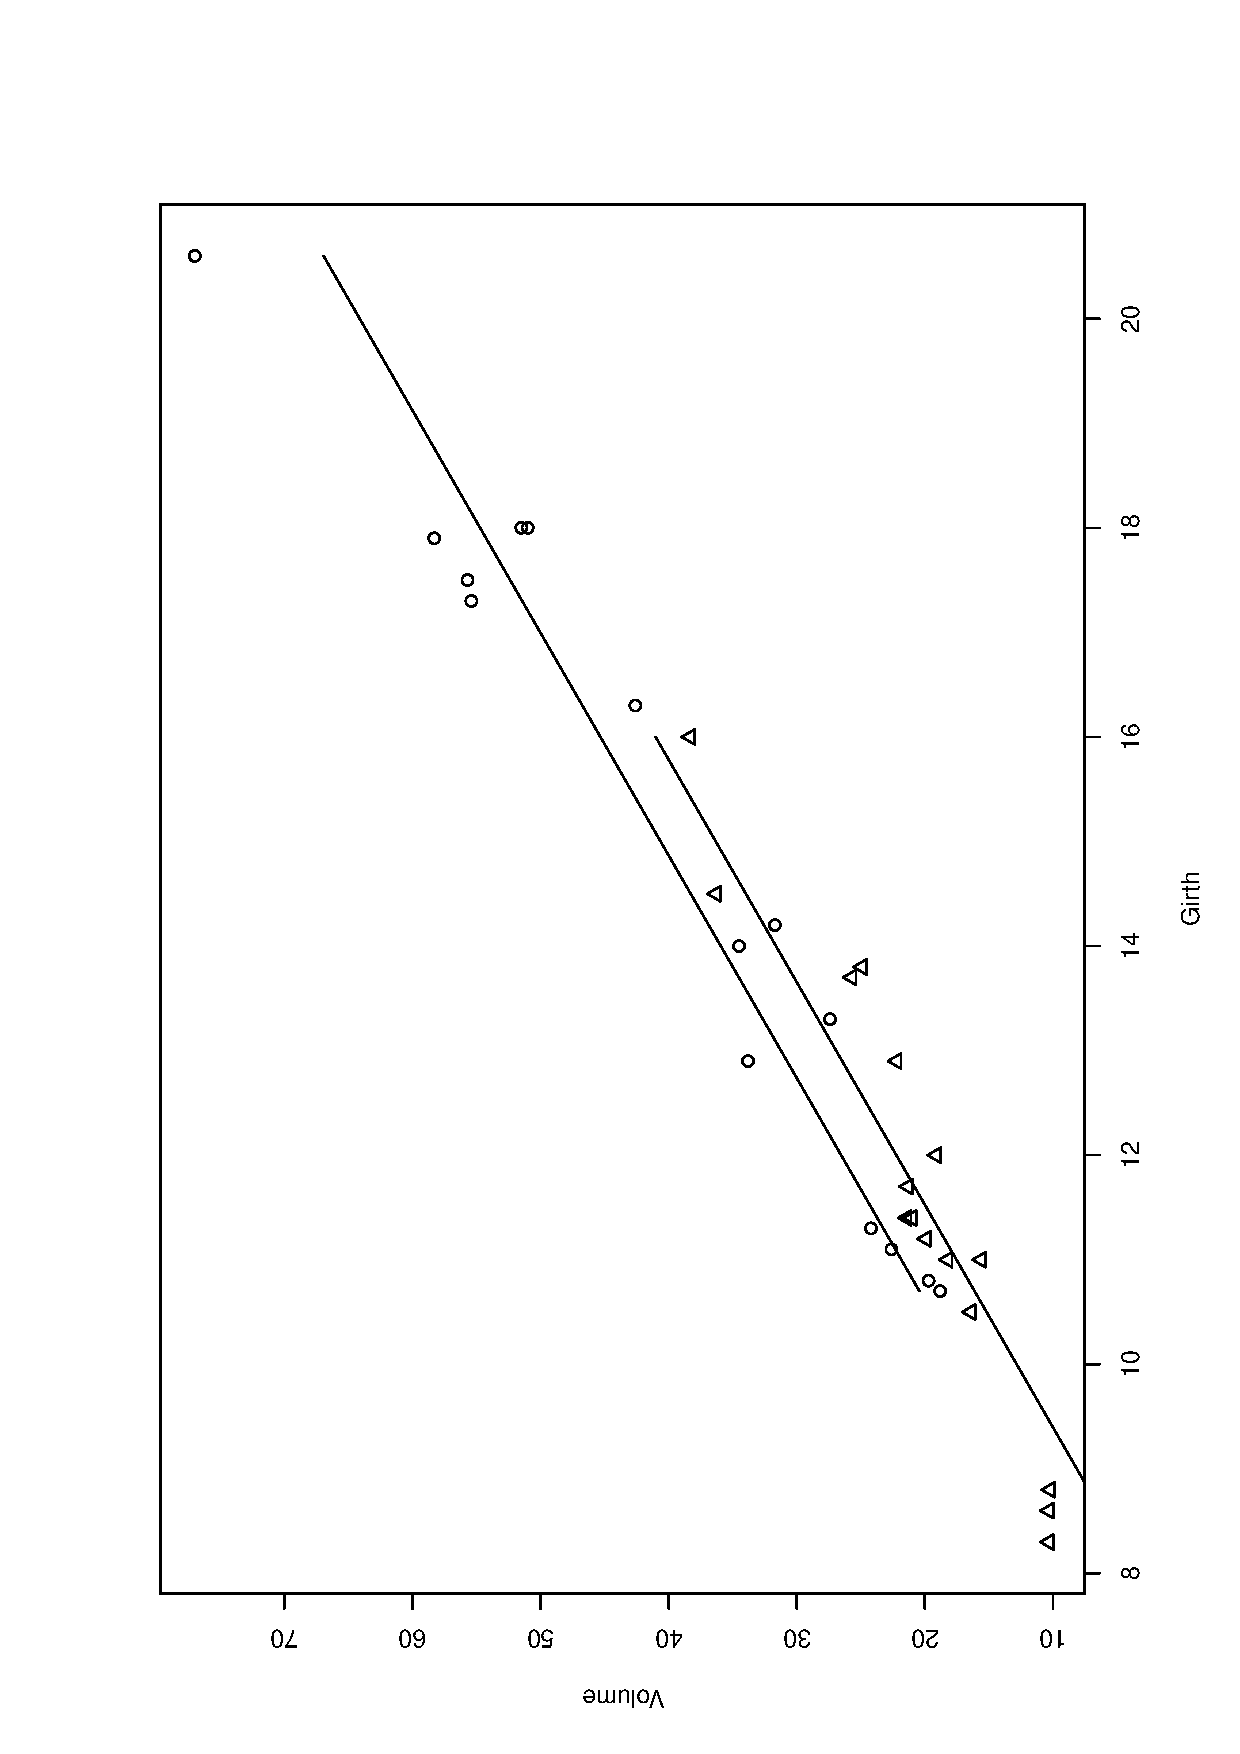
\includegraphics[width=5in, height=4in]{img/dummy-variable-trees.pdf}
    \caption[A dummy variable model for the \texttt{trees} data]{\small A dummy variable model for the \texttt{trees} data.}
    \label{fig:dummy-variable-trees}
  \end{figure}

It may look intimidating but there is reason to the madness. First we \texttt{split} the \texttt{trees} data into two pieces, with groups determined by the \texttt{Tall} variable. Next we add the \texttt{Fit}ted values to each piece via \texttt{predict}. Then we set up a \texttt{plot} for the variables \texttt{Volume} versus \texttt{Girth}, but we do not plot anything yet (\texttt{type = n}) because we want to use different symbols for the two groups. Next we add \texttt{points} to the plot for the \texttt{Tall = yes} trees and use an open circle for a plot character (\texttt{pch = 1}), followed by \texttt{points} for the \texttt{Tall = no} trees with a triangle character (\texttt{pch = 2}). Finally, we add regression \texttt{lines} to the plot, one for each group.

There are other -- shorter -- ways to plot regression lines by groups, namely the \texttt{scatterplot} function in the \texttt{car} \cite{car} package and the \texttt{xyplot} function in the \texttt{lattice} package. We elected to introduce the reader to the above approach since many advanced plots in \textsf{R} are done in a similar, consecutive fashion.
\section{Partial \emph{F} Statistic}
\label{sec-1-7}

\label{sec:Partial-F-Statistic}

We saw in Section \ref{sub:mlr-Overall-F-Test} how to test $H_{0}:\beta_{0}=\beta_{1}=\cdots=\beta_{p}=0$ with the overall $F$ statistic and we saw in Section \ref{sub:mlr-Student's-t-Tests} how to test $H_{0}:\beta_{i}=0$ that a particular coefficient $\beta_{i}$ is zero. Sometimes, however, we would like to test whether a certain part of the model is significant. Consider the regression model
\begin{equation}
Y=\beta_{0}+\beta_{1}x_{1}+\cdots+\beta_{j}x_{j}+\beta_{j+1}x_{j+1}+\cdots+\beta_{p}x_{p}+\epsilon,
\end{equation}
where $j\geq1$ and $p\geq2$. Now we wish to test the hypothesis
\begin{equation}
H_{0}:\beta_{j+1}=\beta_{j+2}=\cdots=\beta_{p}=0
\end{equation}
versus the alternative 
\begin{equation}
H_{1}:\mbox{at least one of \ensuremath{\beta_{j+1},\ \beta_{j+2},\ ,\ldots,\beta_{p}\neq0}}.
\end{equation}

The interpretation of $H_{0}$ is that none of the variables $x_{j+1}$, \ldots{},$x_{p}$ is significantly related to $Y$ and the interpretation of $H_{1}$ is that at least one of $x_{j+1}$, \ldots{},$x_{p}$ is significantly related to $Y$. In essence, for this hypothesis test there are two competing models under consideration:
\begin{align}
\mbox{the full model:} & \quad y=\beta_{0}+\beta_{1}x_{1}+\cdots+\beta_{p}x_{p}+\epsilon,\\
\mbox{the reduced model:} & \quad y=\beta_{0}+\beta_{1}x_{1}+\cdots+\beta_{j}x_{j}+\epsilon,
\end{align}

Of course, the full model will always explain the data \emph{better} than the reduced model, but does the full model explain the data \emph{significantly better} than the reduced model? This question is exactly what the partial $F$ statistic is designed to answer.

We first calculate $SSE_{f}$, the unexplained variation in the full model, and $SSE_{r}$, the unexplained variation in the reduced model. We base our test on the difference $SSE_{r}-SSE_{f}$ which measures the reduction in unexplained variation attributable to the variables $x_{j+1}$, \ldots{}, $x_{p}$. In the full model there are $p+1$ parameters and in the reduced model there are $j+1$ parameters, which gives a difference of $p-j$ parameters (hence degrees of freedom). The partial \emph{F} statistic is 
\begin{equation}
F=\frac{(SSE_{r}-SSE_{f})/(p-j)}{SSE_{f}/(n-p-1)}.
\end{equation}
It can be shown when the regression assumptions hold under $H_{0}$ that the partial $F$ statistic has an $\mathsf{f}(\mathtt{df1}=p-j,\,\mathtt{df2}=n-p-1)$ distribution. We calculate the $p$-value of the observed partial $F$ statistic and reject $H_{0}$ if the $p$-value is small. 


\paragraph*{How to do it with \textsf{R}}

The key ingredient above is that the two competing models are \emph{nested} in the sense that the reduced model is entirely contained within the complete model. The way to test whether the improvement is significant is to compute \texttt{lm} objects both for the complete model and the reduced model then compare the answers with the \texttt{anova} function.

\begin{example}
\label{exa:mlr-trees-poly-no-rescale}

For the \texttt{trees} data, let us fit a polynomial regression model and for the sake of argument we will ignore our own good advice and fail to rescale the explanatory variables. 


\begin{verbatim}
treesfull.lm <- lm(Volume ~ Girth + I(Girth^2) + Height + 
                   I(Height^2), data = trees)
summary(treesfull.lm)
\end{verbatim}


\begin{verbatim}
 
Call:
lm(formula = Volume ~ Girth + I(Girth^2) + Height + I(Height^2), 
    data = trees)

Residuals:
   Min     1Q Median     3Q    Max 
-4.368 -1.670 -0.158  1.792  4.358 

Coefficients:
             Estimate Std. Error t value Pr(>|t|)    
(Intercept) -0.955101  63.013630  -0.015    0.988    
Girth       -2.796569   1.468677  -1.904    0.068 .  
I(Girth^2)   0.265446   0.051689   5.135 2.35e-05 ***
Height       0.119372   1.784588   0.067    0.947    
I(Height^2)  0.001717   0.011905   0.144    0.886    
---
Signif. codes:  0 '***' 0.001 '**' 0.01 '*' 0.05 '.' 0.1 ' ' 1 

Residual standard error: 2.674 on 26 degrees of freedom
Multiple R-squared: 0.9771,	Adjusted R-squared: 0.9735 
F-statistic:   277 on 4 and 26 DF,  p-value: < 2.2e-16
\end{verbatim}

In this ill-formed model nothing is significant except \texttt{Girth} and \texttt{Girth\textasciicircum{}2}. Let us continue down this path and suppose that we would like to try a reduced model which contains nothing but \texttt{Girth} and \texttt{Girth\textasciicircum{}2} (not even an \texttt{Intercept}). Our two models are now
\begin{align*} 
\mbox{the full model:} & \quad Y=\beta_{0}+\beta_{1}x_{1}+\beta_{2}x_{1}^{2}+\beta_{3}x_{2}+\beta_{4}x_{2}^{2}+\epsilon,\\
\mbox{the reduced model:} & \quad Y=\beta_{1}x_{1}+\beta_{2}x_{1}^{2}+\epsilon,
\end{align*}
We fit the reduced model with \texttt{lm} and store the results:


\begin{verbatim}
treesreduced.lm <- lm(Volume ~ -1 + Girth + I(Girth^2), data = trees)
\end{verbatim}

To delete the intercept from the model we used \texttt{-1} in the model formula. Next we compare the two models with the \texttt{anova} function. The convention is to list the models from smallest to largest.


\begin{verbatim}
anova(treesreduced.lm, treesfull.lm)
\end{verbatim}

\begin{verbatim}
 Analysis of Variance Table
 
 Model 1: Volume ~ -1 + Girth + I(Girth^2)
 Model 2: Volume ~ Girth + I(Girth^2) + Height + I(Height^2)
   Res.Df    RSS Df Sum of Sq      F   Pr(>F)   
 1     29 321.65                                
 2     26 185.86  3    135.79 6.3319 0.002279 **
 ---
 Signif. codes:  0 '***' 0.001 '**' 0.01 '*' 0.05 '.' 0.1 ' ' 1
\end{verbatim}

We see from the output that the complete model is highly significant compared to the model that does not incorporate \texttt{Height} or the \texttt{Intercept}. We wonder (with our tongue in our cheek) if the \texttt{Height\textasciicircum{}2} term in the full model is causing all of the trouble. We will fit an alternative reduced model that only deletes \texttt{Height\textasciicircum{}2}. 


\begin{verbatim}
treesreduced2.lm <- lm(Volume ~ Girth + I(Girth^2) + Height, 
                       data = trees)
anova(treesreduced2.lm, treesfull.lm)
\end{verbatim}

\begin{verbatim}
  Analysis of Variance Table
 
 Model 1: Volume ~ Girth + I(Girth^2) + Height
 Model 2: Volume ~ Girth + I(Girth^2) + Height + I(Height^2)
   Res.Df    RSS Df Sum of Sq      F Pr(>F)
 1     27 186.01                           
 2     26 185.86  1   0.14865 0.0208 0.8865
\end{verbatim}

In this case, the improvement to the reduced model that is attributable to \texttt{Height\textasciicircum{}2} is not significant, so we can delete \texttt{Height\textasciicircum{}2} from the model with a clear conscience. We notice that the \emph{p-value} for this latest partial $F$ test is 0.8865, which seems to be remarkably close to the \emph{p-value} we saw for the univariate \emph{t} test of \texttt{Height\textasciicircum{}2} at the beginning of this example. In fact, the \emph{p-values} are \emph{exactly} the same. Perhaps now we gain some insight into the true meaning of the univariate tests.

\end{example}
\section{Residual Analysis and Diagnostic Tools}
\label{sec-1-8}

\label{sec:Residual-Analysis-MLR}

We encountered many, many diagnostic measures for simple linear regression in Sections \ref{sec:Residual-Analysis-SLR} and \ref{sec:Other-Diagnostic-Tools-SLR}. All of these are valid in multiple linear regression, too, but there are some slight changes that we need to make for the multivariate case. We list these below, and apply them to the trees example.  

\begin{description}
\item[Shapiro-Wilk, Breusch-Pagan, Durbin-Watson:] unchanged from SLR, but we are now equipped to talk about the Shapiro-Wilk test statistic for the residuals. It is defined by the formula 
   \begin{equation}
   W=\frac{\mathbf{a}^{\mathrm{T}}\mathbf{E}^{\ast}}{\mathbf{E}^{\mathrm{T}}\mathbf{E}},
   \end{equation}
   where $\mathbf{E}^{\ast}$ is the sorted residuals and $\mathbf{a}_{1\times\mathrm{n}}$ is defined by 
   \begin{equation}
   \mathbf{a}=\frac{\mathbf{m}^{\mathrm{T}}\mathbf{V}^{-1}}{\sqrt{\mathbf{m}^{\mathrm{T}}\mathbf{V}^{-1}\mathbf{V}^{-1}\mathbf{m}}},
   \end{equation}
   where $\mathbf{m}_{\mathrm{n}\times1}$ and $\mathbf{V}_{\mathrm{n}\times\mathrm{n}}$ are the mean and covariance matrix, respectively, of the order statistics from an $\mathsf{mvnorm}\left(\mathtt{mean}=\mathbf{0},\,\mathtt{sigma}=\mathbf{I}\right)$ distribution.
\item[Leverages:] are defined to be the diagonal entries of the hat matrix $\mathbf{H}$ (which is why we called them $h_{ii}$ in Section \ref{sub:mlr-point-est-regsurface}). The sum of the leverages is $\mbox{tr}(\mathbf{H})=p+1$. One rule of thumb considers a leverage extreme if it is larger than double the mean leverage value, which is $2(p+1)/n$, and another rule of thumb considers leverages bigger than 0.5 to indicate high leverage, while values between 0.3 and 0.5 indicate moderate leverage.
\item[Standardized residuals:] unchanged. Considered extreme if $|R_{i}|>2$.
\item[Studentized residuals:] compared to a $\mathsf{t}(\mathtt{df}=n-p-2)$ distribution.
\item[DFBETAS:] The formula is generalized to
   \begin{equation}
   (DFBETAS)_{j(i)}=\frac{b_{j}-b_{j(i)}}{S_{(i)}\sqrt{c_{jj}}},\quad j=0,\ldots p,\ i=1,\ldots,n,
   \end{equation}
   where $c_{jj}$ is the $j^{\mathrm{th}}$ diagonal entry of $(\mathbf{X}^{\mathrm{T}}\mathbf{X})^{-1}$. Values larger than one for small data sets or $2/\sqrt{n}$ for large data sets should be investigated.
\item[DFFITS:] unchanged. Larger than one in absolute value is considered extreme.
\item[Cook's D:] compared to an $\mathsf{f}(\mathtt{df1}=p+1,\,\mathtt{df2}=n-p-1)$ distribution. Observations falling higher than the 50$^{\textrm{th}}$ percentile are extreme.
\end{description}
Note that plugging the value $p=1$ into the formulas will recover all of the ones we saw in Chapter \ref{cha:simple-linear-regression}.
\section{Additional Topics}
\label{sec-1-9}

\label{sec:Additional-Topics-MLR}
\subsection{Nonlinear Regression}
\label{sec-1-9-1}


We spent the entire chapter talking about the \texttt{trees} data, and all of our models looked like \texttt{Volume \textasciitilde{} Girth + Height} or a variant of this model. But let us think again: we know from elementary school that the volume of a rectangle is $V=lwh$ and the volume of a cylinder (which is closer to what a black cherry tree looks like) is
\begin{equation}
V=\pi r^{2}h\quad\mbox{or}\quad V=4\pi dh,
\end{equation}
where $r$ and $d$ represent the radius and diameter of the tree, respectively. With this in mind, it would seem that a more appropriate model for $\mu$ might be
\begin{equation}
\mu(x_{1},x_{2})=\beta_{0}x_{1}^{\beta_{1}}x_{2}^{\beta_{2}},\label{eq:trees-nonlin-reg}
\end{equation}
where $\beta_{1}$ and $\beta_{2}$ are parameters to adjust for the fact that a black cherry tree is not a perfect cylinder.

How can we fit this model? The model is not linear in the parameters any more, so our linear regression methods will not work\ldots{} or will they? In the \texttt{trees} example we may take the logarithm of both sides of Equation \ref{eq:trees-nonlin-reg} to get
\begin{equation}
\mu^{\ast}(x_{1},x_{2})=\ln\left[\mu(x_{1},x_{2})\right]=\ln\beta_{0}+\beta_{1}\ln x_{1}+\beta_{2}\ln x_{2},
\end{equation}
and this new model $\mu^{\ast}$ is linear in the parameters $\beta_{0}^{\ast}=\ln\beta_{0}$, $\beta_{1}^{\ast}=\beta_{1}$ and $\beta_{2}^{\ast}=\beta_{2}$. We can use what we have learned to fit a linear model \texttt{log(Volume) \textasciitilde{} log(Girth) + log(Height)}, and everything will proceed as before, with one exception: we will need to be mindful when it comes time to make predictions because the model will have been fit on the log scale, and we will need to transform our predictions back to the original scale (by exponentiating with \texttt{exp}) to make sense.


\begin{verbatim}
treesNonlin.lm <- lm(log(Volume) ~ log(Girth) + log(Height), 
                     data = trees)
summary(treesNonlin.lm)
\end{verbatim}


\begin{verbatim}
 
Call:
lm(formula = log(Volume) ~ log(Girth) + log(Height), data = trees)

Residuals:
      Min        1Q    Median        3Q       Max 
-0.168561 -0.048488  0.002431  0.063637  0.129223 

Coefficients:
            Estimate Std. Error t value Pr(>|t|)    
(Intercept) -6.63162    0.79979  -8.292 5.06e-09 ***
log(Girth)   1.98265    0.07501  26.432  < 2e-16 ***
log(Height)  1.11712    0.20444   5.464 7.81e-06 ***
---
Signif. codes:  0 '***' 0.001 '**' 0.01 '*' 0.05 '.' 0.1 ' ' 1 

Residual standard error: 0.08139 on 28 degrees of freedom
Multiple R-squared: 0.9777,	Adjusted R-squared: 0.9761 
F-statistic: 613.2 on 2 and 28 DF,  p-value: < 2.2e-16
\end{verbatim}

This is our best model yet (judging by $R^{2}$ and $\overline{R}^{2}$), all of the parameters are significant, it is simpler than the quadratic or interaction models, and it even makes theoretical sense. It rarely gets any better than that.

We may get confidence intervals for the parameters, but remember that it is usually better to transform back to the original scale for interpretation purposes :


\begin{verbatim}
exp(confint(treesNonlin.lm))
\end{verbatim}

\begin{verbatim}
                    2.5 %      97.5 %
 (Intercept) 0.0002561078 0.006783093
 log(Girth)  6.2276411645 8.468066317
 log(Height) 2.0104387829 4.645475188
\end{verbatim}

(Note that we did not update the row labels of the matrix to show that we exponentiated and so they are misleading as written.) We do predictions just as before. Remember to transform the response variable back to the original scale after prediction. 


\begin{verbatim}
new <- data.frame(Girth = c(9.1, 11.6, 12.5), Height = c(69, 74, 87))
exp(predict(treesNonlin.lm, newdata = new, interval = "confidence"))
\end{verbatim}

\begin{verbatim}
        fit      lwr      upr
 1 11.90117 11.25908 12.57989
 2 20.82261 20.14652 21.52139
 3 28.93317 27.03755 30.96169
\end{verbatim}

The predictions and intervals are slightly different from those calculated earlier, but they are close. Note that we did not need to transform the \texttt{Girth} and \texttt{Height} arguments in the dataframe \texttt{new}. All transformations are done for us automatically.
\subsection{Real Nonlinear Regression}
\label{sec-1-9-2}


We saw with the \texttt{trees} data that a nonlinear model might be more appropriate for the data based on theoretical considerations, and we were lucky because the functional form of $\mu$ allowed us to take logarithms to transform the nonlinear model to a linear one. The same trick will not work in other circumstances, however. We need techniques to fit general models of the form
\begin{equation}
\mathbf{Y}=\mu(\mathbf{X})+\epsilon,
\end{equation}
where $\mu$ is some crazy function that does not lend itself to linear transformations.

There are a host of methods to address problems like these which are studied in advanced regression classes. The interested reader should see Neter \emph{et al} \cite{Neter1996} or Tabachnick and Fidell \cite{Tabachnick2006}. 

It turns out that John Fox has posted an Appendix to his book \cite{Fox2002} which discusses some of the methods and issues associated with nonlinear regression; see \href{http://cran.r-project.org/doc/contrib/Fox-Companion/appendix.html}{here} for more.  Here is an example of how it works, based on a question from R-help.


\begin{verbatim}
# fake data 
set.seed(1) 
x <- seq(from = 0, to = 1000, length.out = 200) 
y <- 1 + 2*(sin((2*pi*x/360) - 3))^2 + rnorm(200, sd = 2)
# plot(x, y)
acc.nls <- nls(y ~ a + b*(sin((2*pi*x/360) - c))^2, 
               start = list(a = 0.9, b = 2.3, c = 2.9))
summary(acc.nls)
#plot(x, fitted(acc.nls))
\end{verbatim}


\begin{verbatim}
 
Formula: y ~ a + b * (sin((2 * pi * x/360) - c))^2

Parameters:
  Estimate Std. Error t value Pr(>|t|)    
a  0.95884    0.23097   4.151 4.92e-05 ***
b  2.22868    0.37114   6.005 9.07e-09 ***
c  3.04343    0.08434  36.084  < 2e-16 ***
---
Signif. codes:  0 '***' 0.001 '**' 0.01 '*' 0.05 '.' 0.1 ' ' 1 

Residual standard error: 1.865 on 197 degrees of freedom

Number of iterations to convergence: 3 
Achieved convergence tolerance: 6.546e-08
\end{verbatim}
\subsection{Multicollinearity}
\label{sec-1-9-3}

\label{sub:Multicollinearity}

A multiple regression model exhibits \emph{multicollinearity} when two or more of the explanatory variables are substantially correlated with each other. We can measure multicollinearity by having one of the explanatory play the role of ``dependent variable'' and regress it on the remaining explanatory variables. The the $R^{2}$ of the resulting model is near one, then we say that the model is multicollinear or shows multicollinearity.

Multicollinearity is a problem because it causes instability in the regression model. The instability is a consequence of redundancy in the explanatory variables: a high $R^{2}$ indicates a strong dependence between the selected independent variable and the others. The redundant information inflates the variance of the parameter estimates which can cause them to be statistically insignificant when they would have been significant otherwise. To wit, multicollinearity is usually measured by what are called \emph{variance inflation factors}.

Once multicollinearity has been diagnosed there are several approaches to remediate it. Here are a couple of important ones. 

\begin{description}
\item[Principal Components Analysis.] This approach casts out two or more of the original explanatory variables and replaces them with new variables, derived from the original ones, that are by design uncorrelated with one another. The redundancy is thus eliminated and we may proceed as usual with the new variables in hand. Principal Components Analysis is important for other reasons, too, not just for fixing multicollinearity problems.
\item[Ridge Regression.] The idea of this approach is to replace the original parameter estimates with a different type of parameter estimate which is more stable under multicollinearity. The estimators are not found by ordinary least squares but rather a different optimization procedure which incorporates the variance inflation factor information.
\end{description}

We decided to omit a thorough discussion of multicollinearity because we are not equipped to handle the mathematical details. Perhaps the topic will receive more attention in a later edition.

\begin{itemize}
\item What to do when data are not normal
\begin{itemize}
\item Bootstrap (see Chapter \ref{cha:resampling-methods}).
\end{itemize}
\end{itemize}
\subsection{Akaike's Information Criterion}
\label{sec-1-9-4}


\[
AIC=-2\ln L+2(p+1)
\]

\newpage{}
\section{Chapter Exercises}
\label{sec-1-10}


\addcontentsline{toc}{section}{Chapter Exercises}
\setcounter{thm}{0}

\begin{xca}
\label{xca:anova-equality}
Use Equations \ref{eq:mlr-sse-matrix}, \ref{eq:mlr-ssto-matrix}, and \ref{eq:mlr-ssr-matrix} to prove the Anova Equality:
\[
SSTO=SSE+SSR.
\]
\end{xca}

\end{document}